\chapter{Models of Computation}
\label{cha:models}


A \emph{model of computation} describes what computation is and how it
is done. The best known is Alan Turing's
model~\sidecite{turing37:_comput_number_with_applic_to_entsc} in which a
machine manipulates the contents of a tape according to a finite set
of instructions. It has become the yardstick with which we measure
other models of computation. Turing's notion of computability is very
robust. Firstly, it is robust because changes to the definition of
Turing machines, such as increasing the number of tapes or heads, or
allowing the head to jump around, does not change the computational
power. Secondly, the notion is robust because many other definitions
of computation turned out to be equivalent to Turing's in the sense
that machines of one kind can simulate those of the other kind, and
vice versa.

However, we would commit a serious mistake if we concluded that by
studying only Turing machines we will learn everything there is to
learn about computable mathematics. Our inquiry into the nature of
computation, especially computation with infinite structures, will
reveal a plethora of possibilities which are \emph{not} equivalent.
Thus we begin the chapter with a review of several models of
computation, which then leads us to a general definition of
computational models.


\section{Turing machines}
\label{sec:turing-machines}

We recall informally how a Turing machine operates. There is little
point in giving a formal definition because we do not intend to
actually write programs for Turing machines. If you are not familiar
with Turing machines we recommend one of standard textbooks on the
subject~\sidecite{odifreddi89:_class_recur_theor,h.r.92:_theor_recur_funct_effec_comput,davis58:_comput_unsol}.

\begin{figure}[htbp]
  \centering
  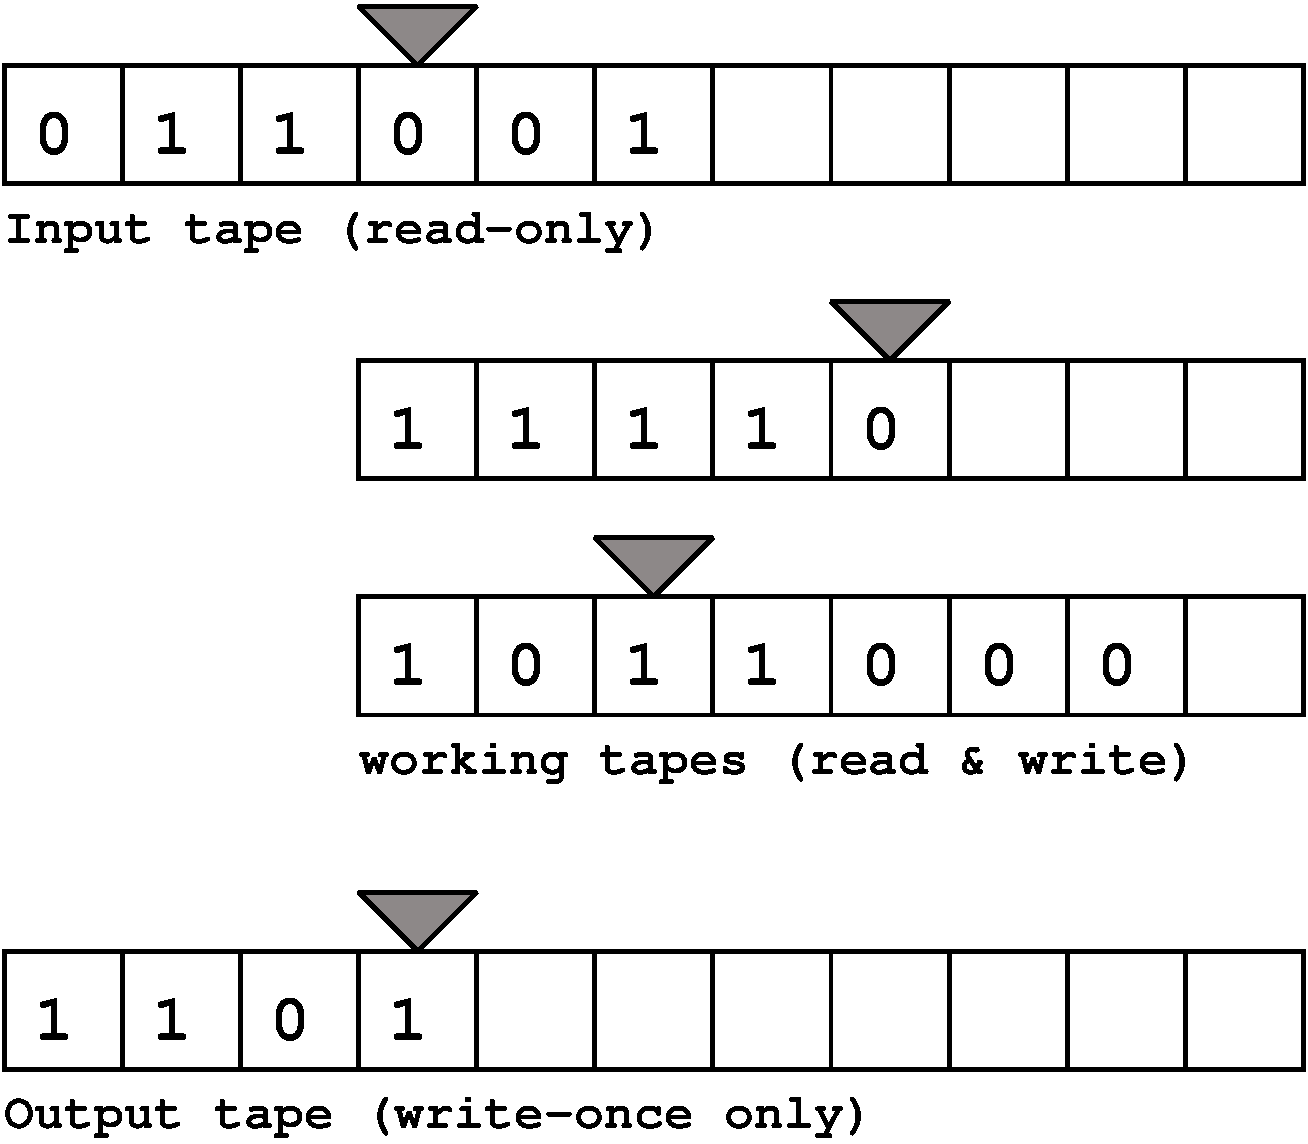
\includegraphics[width=0.5\textwidth]{turing_machine}
  \caption{A Turing machine operates with tapes}
  \label{fig:turing-machine}
\end{figure}

A Turing machine is a device which operates on a number of tapes and
heads, see Figure~\ref{fig:turing-machine}:
%
\begin{itemize}
\item the input tape is equipped with a reading head that can move
  left and right, and read the symbols, but cannot write them.
\item The working tapes are equipped with heads that move left and
  right, and can both read and write symbols.
\item The output tape is equipped with a write-once head which can
  move left and right, and it can write into each cell exactly once.
  Once a cell is filled with a non-blank symbol all subsequent writes
  to it are ignored.
\end{itemize}
%
The tapes are infinite\sidenote{If you are worried about having actual
  infinite tapes in your room, note that at each step of the
  computation only a finite portion of tapes has been inspected. In
  this sense the tapes are \emph{potentially} infinite.} and contain
symbols from a given finite alphabet. A common choice for the alphabet
is $0$, $1$, and a special symbol `blank'. The machine manipulates the
contents of the tapes according to a \emph{program}, which is a finite
list of simple instructions that control the heads and the tapes. The
machine executes one instruction at a time in a sequential manner. It
may \emph{terminate} after having executed finitely many computation
steps. If it does not terminate then it runs forever, in which case we
say that it \emph{diverges}.

Our version of Turing machine is different from the usual one, where a
machine is equipped with only a single tape that serves for input,
output, and intermediate work. The two formulations are equivalent in
the sense that a single-tape machine can simulate the workings of a
Turing machine with several tapes, and vice versa. Our variant will
ease the description of infinite computations in
Section~\ref{sec:type-2}.

The state of a Turing machine may be encoded onto a single tape as
follows. First we write down the program, suitably encoded by the
symbols from the alphabet, then the current state (the next
instruction to be executed), and positions of the heads. Finally, we
copy the contents of all the tapes by interleaving them into a single
tape.

If we were going to build just one machine, which one would we build?
The answer was given by Turing.

\begin{theorem}[Turing]
  \label{thm:universal-machine}
  There exists a \defemph{universal  machine}---a machine that takes a
  description of another machine, as explained above, and simulates
  it.
\end{theorem}

\begin{proof}
  A traditional proof may be found in any book on computability
  theory, and there is nothing wrong with reading the original
  proof~\sidecite{turing37:_comput_number_with_applic_to_entsc} either.
  For me a much more convincing proof is the fact that a universal
  machine is sitting right here on my desk. (You have to
    ignore the fact that several hundred gigabytes of storage are not
    quite the same thing as an infinite tape. Also, modern computers
    are really \emph{Von Neumann}
    machines~\sidecite{goldstein47:_repor_mathem_and_logic_aspec} because
    they have a central processing unit and random access memory
    instead of a tape.)
\end{proof}

Once we have a universal machine, we can make it behave like any other
machine. It is just
\href{http://www.catb.org/jargon/html/S/SMOP.html}{``a simple matter
  of programming''} to tell it what to do.

We mentioned in the introduction that many kinds of computing devices
are equivalent to Turing machines. We shall therefore not insist on
describing computation solely in terms of Turing machines, but rather
rely on familiarity with modern computers and programming languages.
After all, programs can actually be run on computers, whereas Turing
machines are hard to get by.


\subsection{Type 1 machines}
\label{sec:type-1}

How do we use Turing machines to compute a partial function $f :
\NN \parto \NN$? A natural idea is to write the argument $n$ onto the
input tape, run the machine until it terminates, and read the result
$f(n)$ off the output tape. If the machine diverges then $f(n)$ is
undefined. Of course, the input $n$ must be suitably encoded onto the
input tape, for example it can be written in binary form. The output
tape contains the result encoded in the same manner.

It is convenient to view every Turing machine as one computing a
function $\NN \parto \NN$. This can be arranged as long as we read the
result off the output tape correctly. Suppose the alphabet contains
symbols $0$, $1$, and blank. We encode the input $n$ onto the input
tape in binary followed by blanks, and run the machine. If and when it
terminates it has written at most finally many symbols onto the output
tape. Some of the symbols it has written might be different from $0$
and $1$. If we ignore everything that comes after the first blank, we
can interpret the output tape as a number written in binary (the empty
sequence encodes zero).

We could similarly define how a Turing machine computes a multivariate
partial function $f : \NN^k \parto \NN$. We just have to correctly
encode the arguments on the tape by placing special markers between
them so that we can tell where one ends and the next one begins.

It is common knowledge that computers encode everything with $0$'s and
$1$'s, but logicians prefer to encode everything with natural numbers.
We shall write in general $\code{e}$ for encoding of $e$ by a natural
number. Of course, we must specify what $\code{e}$ is in each
particular case. For example, a pair of numbers $(m, n)$ may be
encoded into a single number as
%
\begin{equation*}
  \code{(m, n)} = 2^m (2 n + 1).
\end{equation*}
%
Every number except $0$ represents the code of a unique pair so we
also have computable \defemph{projections} $\xfst$ and $\xsnd$ which
recover $m$ and $n$ from $\code{(m, n)}$, respectively.

We may also encode Turing machines with numbers. A program is a finite
list of instructions, so it can be encoded as a finite sequence of
$0$'s and $1$'s (your computer does this every time you save a piece of
source code in a file), which in turn represents a number in binary
form. In fact, every number may be thought of as a code of a program
by the reverse process. Given a number, write it in binary form and
interpret it as a sequence of $0$'s and $1$'s and decode from it a
list of instructions. It may happen that the binary sequence does not
properly encode a list of instructions, in which case we interpret it
as the program that keeps moving the input head to the right forever.

The next step is to encode tapes and entire computations with numbers.
Because an infinite tape cannot be encoded in a single natural number,
we limit attention to the so-called \emph{type 1} machines which
accept only \emph{finite} inputs. More precisely, the input always
consists of a finite string of $0$'s and $1$'s followed by blanks.
Such input may be encoded by a single number. Furthermore, at every
step of computation the machine has used up only a finite portion of
its working tapes. The contents of each tape may be encoded by a
single number, and a finite sequence of numbers $[n_0, \ldots, n_k]$
may again be encoded by a single number $\code{[n_0, \ldots, n_k]}$,
which we define as iterated pairing:
%
\begin{align*}
  \code{[\;]} &= 0 \\
  \code{[n_0, \ldots, n_k]} &= \code{(n_0, \code{[n_1, \ldots, n_k]})}.
\end{align*}
%
Because we defined $\code{(m,n)}$ so that it is never zero, the
elements of a sequence may be uniquely reconstructed from its code. By
continuing in this manner we may encode with a single number a finite
sequence of computation steps, including the contents of the tapes
and positions of the heads at each step. Stephen Kleene~\sidecite{kleene43:_recur_predic_and_quant}
worked out the details of all this and defined the predicate
$T(x,y,z)$ whose meaning is
%
\begin{quote}
  ``Machine encoded by $x$ with input tape that encodes the number $y$
  performs a sequence of computation steps encoded by $z$ and
  terminates.''
\end{quote}
%
The amazing thing is that $T$ may be defined in Peano arithmetic just
in terms of basic arithmetical operations on numbers. There is an
associated computable partial function $U(z)$ whose meaning is ``the
number encoded by the contents of the output tape in the last step of
computation encoded by $z$''. The function $U$ allows us to extract
the result of a computation. If $z$ does not encode a terminating
computation then $U(z)$ is undefined.

Kleene's normal form theorem~\sidecite{kleene43:_recur_predic_and_quant}
says that every partial computable function $f : \NN \parto \NN$ may
be written in the form
%
\begin{equation}
  \label{eq:kleene-normal-form}
  y \mapsto U(\min \set{z \in \NN \such T(x,y,z)}).
\end{equation}
%
The number $x$ is the encoding of any machine that computes~$f$. We
emphasize that we are completely ignoring questions of computational
efficiency. Just consider how we would compute $f(y)$ according
to~\eqref{eq:kleene-normal-form}: for each $z = 0, 1, 2, \ldots$, test
whether~$z$ encodes a computation of machine $x$ with input $y$. When
you find the first such~$z$, extract the result $U(z)$ from it. I dare
you to compute the identity function $y \mapsto y$ this way!

Kleene's normal form may be used to define a standard enumeration of
partial recursive functions. Let
%
\begin{equation*}
  \pr{x}{y} = U(\min \set{z \in \NN \such T(x,y,z)}).
\end{equation*}
%
The sequence $\xpr_0, \xpr_1, \xpr_2, \ldots$ is an enumeration of all
computable partial functions (with repetitions).

The preceding discussion may be generalized to functions of several
variables. For each $k \in \NN$ there is Kleene's predicate
$T^{(k)}(x,y_1,\ldots,y_k,z)$ and the corresponding $U^{(k)}(z)$ that
extracts results from computations. Similarly, there is a standard
enumeration of $k$-place computable partial functions
%
\begin{equation*}
  \prm{k}{x}{y_1, \ldots, y_k} =
  U^{(k)}(\min \set{z \in \NN \such T^{(k)}(x,y_1, \ldots, y_k,z)}).
\end{equation*}
%
These enumerations are not arbitrary, because they have the following
important properties.

\begin{theorem}[utm]
  There exists a partial computable function $u : \NN \times
  \NN \parto \NN$ such that, for all $x, y \in \NN$,
  %
  \begin{equation*}
    u(x,y) \simeq \pr{x}{y}.
  \end{equation*}
\end{theorem}

\begin{theorem}[smn]
  There exists a computable function $s :
  \NN^2 \to \NN$ such that, for all $x, y, z \in \NN$,
  %
  \begin{equation*}
    \pr{s(x, y)}{z} \simeq \prm{2}{x}{y,z}.
  \end{equation*}
\end{theorem}

\noindent
The utm theorem is essentially a restatement of
Theorem~\ref{thm:universal-machine} in terms of computable partial
functions. A detailed proof of the utm and smn theorems would involve
a lot of technical manipulations of Turing machines. Rather than
losing time with such a historical exercise, let us see how these two
theorems manifest themselves in modern programming languages, say in
Haskell. Keeping in mind that numbers are just codes for programs and
data, the universal function $u$ from the utm theorem is
%
\begin{lstlisting}[language=Haskell]
u (f, y) = f y
\end{lstlisting}
%
and the function $s$ is the currying operation\sidenote{In Haskell the
  notation \texttt{{\char92}x -> e} stands for $\lambda$-abstraction
  $\lam{x}{e}$, which in turn means ``the function which maps $x$ to
  $e$'', see Section~\ref{sec:lambda-calculus}.}
%
\begin{lstlisting}[language=Haskell]
s (f, y) = \z -> f (y, z)
\end{lstlisting}
%
This may seem like a triviality to the programmer but is surely not
considered one by those who implemented the Haskell compiler. The
operation that we used to define \lstinline!s! are application,
pairing, currying and $\lambda$-abstraction. They are ``the essence''
of functional programming, just like the utm and smn theorems are the
essence of partial computable functions.

The following theorem is important in the theory of computable
functions because it allows us to define partial computable functions
by recursion.

\begin{theorem}[Recursion theorem]
  For every \emph{total} computable $f : \NN \to \NN$ there exists $x
  \in \NN$ such that $\xpr_{f(n)} = \xpr_{n}$.
\end{theorem}

\begin{proof}
  The classical proof goes as follows. First we define a computable
  partial map $\psi : \NN^2 \parto \NN$ such that
  %
  \begin{equation*}
    \psi(u, x) =
    \begin{cases}
      \pr{\pr{u}{u}}{x} & \text{if $\defined{\pr{u}{u}}$,}\\
      \text{undefined}  & \text{otherwise.}\\
    \end{cases}
  \end{equation*}
  %
  By the smn theorem there is a computable function $g : \NN \to \NN$
  such that $\pr{g(u)}{x} = \psi(u, x)$. Now consider any computable
  $f : \NN \to \NN$. Because $f \circ g$ is computable, there exists
  $v \in \NN$ such that $\xpr_{v} = f \circ g$. Since $f \circ g$ is a
  total function, $\pr{v}{v}$ is defined. The number $n = g(v)$ has
  the desired property:
  $\xpr_{g(v)} = \xpr_{\pr{v}{v}} = \xpr_{f(g(v))} = \xpr_{f(n)}$.
\end{proof}

This was a typical argument in the theory of computable functions. Let
us prove the recursion theorem in Haskell to see what is going on. The
function $f : \NN \to \NN$ operates on codes of computable partial
maps. In Haskell we work directly with values, so in the Haskell
version of the theorem $f$ has the type
%
\begin{lstlisting}[language=Haskell]
f :: (Integer -> Integer) -> (Integer -> Integer)
\end{lstlisting}
%
Rather than looking for a number $n$ we are looking for a function
\lstinline!n! such that \lstinline!f n = n!. Because Haskell already
has recursion built in this is very easy, just define
%
\begin{lstlisting}
n = f n
\end{lstlisting}
%
Recursion theorem accomplishes for type~1 machines what is already
built into general-purpose programming language, namely definition by
recursion.

We finish this section with a theorem which we shall often use to show
\emph{non}-computability results.

\begin{theorem}[Halting oracle]
  The \defemph{halting oracle},
  %
  \begin{equation*}
    h(x) =
    \begin{cases}
      1 & \text{if $\pr{x}{0}$ is defined,}\\
      0 & \text{if $\pr{x}{0}$ is not defined,}
    \end{cases}
  \end{equation*}
  %
  is \emph{not} computable.
\end{theorem}

\begin{proof}
  Let us prove the theorem in Haskell. We must show that there is no
  %
  \begin{lstlisting}[language=Haskell]
h :: (Integer -> Integer) -> Integer
  \end{lstlisting}
  %
  such that, for all \lstinline!f :: Integer -> Integer!,
  %
  \begin{equation*}
    \text{\lstinline!h f!} =
    \begin{cases}
      \text{\lstinline!1!} & \text{if \lstinline!f 0! terminates,}\\
      \text{\lstinline!0!} & \text{if \lstinline!f 0! diverges.}
    \end{cases}
  \end{equation*}
  %
  Suppose there were such an \lstinline!h!. Define
  %
  \begin{lstlisting}[language=Haskell]
g n = if h g == 1 then g n else 0
  \end{lstlisting}
  %
  By assumption \lstinline!h g! is either \lstinline!0! or
  \lstinline!1!. In either case there is a contradiction because
  \lstinline!g! does just the opposite of what \lstinline!h! says it
  will do.
\end{proof}

\subsection{Type 2 machines}
\label{sec:type-2}

Type 1 machines from previous section only operate on finite inputs.
In practice we often see programs whose input and output are
(potentially) infinite. For example, when you listen to an Internet
radio station, the player accepts a never-ending stream of data which
it outputs to the speakers. Also, just because a program does not
terminate that does not automatically mean it is useless. We therefore
also need a model of computation that describes non-terminating
programs with infinite inputs and outputs.

A popular one is \emph{type 2} Turing machine, which accepts an
infinite sequence on its input tape and is allowed to work forever. It
may or may not fill the output tape entirely with non-blank symbols.
Note that the requirement for the output tape to be write-once makes
it possible to tell when the machine has actually produced an output
in a given cell. Had we allowed the machine to write to each output
cell many times, it could keep coming back and changing what it has
already written.

An important distinction between type 1 and type 2 machines is that
the latter may accept non-computable inputs, from which non-computable
outputs may be produced.

For type 2 machines there are analogues of the standard
enumeration~$\xpr$, utm and the smn theorems. These are more easily
expressed if we allow the machines to write natural numbers in the
cells, rather than symbols from a finite alphabet. We also equip the
machines with instructions for manipulating numbers, say, instructions
for extracting the bits and for testing equality with zero. These
changes are inessential because an infinite sequence $n_0, n_1, n_2,
\ldots$ of natural numbers may be encoded as a binary sequence
$1^{n_0}01^{n_1}01^{n_2}0\cdots$, where $1^k$ means that the symbol
$1$ is repeated $k$-times.

A type 2 machine computes a partial function $f : \NNNN \parto
\NNNN$, where $\NNNN$ is the \defemph{Baire space} of infinite
sequences of numbers. We run the machine with $\alpha \in \NNNN$
written on the input tape. If every output cell is eventually written
to, then the output tape represents the result $f(\alpha)$. If there is
at least one output cell to which the machine does not write a number,
then $f(\alpha)$ is undefined.

We may similarly define what it means for a machine to compute a
multivariate partial function $f : (\NNNN)^k \parto \NNNN$. The
input $(\alpha_0, \ldots, \alpha_{k-1})$ is written onto the input tape in
an interleaving manner, so that $\alpha_i(j)$ is found in the cell at
position $k \cdot j + i$.

Before proceeding with type 2 computability, we recall a few basic
facts about the Baire space~$\Baire = \NNNN$. Let $\NN^{*}$ be the
set of all finite sequences of natural numbers. If $a, b \in \NN^{*}$
we write $a \sqsubseteq b$ when $a$ is a prefix of~$b$. The length of
a finite sequence $a$ is denoted by~$|a|$. Similarly, we write $a
\sqsubseteq \alpha$ when $a$ is a prefix of an infinite sequence
$\alpha \in \Baire$. Define $\seg{a}{n} = [\alpha(0), \ldots,
\alpha(n-1)]$ to be the prefix of~$\alpha$ consisting of the
first~$n$ terms.

The expression $\cons{n}{\alpha}$ denotes the sequence $n, \alpha(0),
\alpha(1), \alpha(2), \ldots$, while $\append{a}{\beta}$ denotes the
concatenation of the finite sequence $a \in \NN^{*}$ with the infinite
sequence $\beta \in \Baire$.

We equip $\Baire$ with the product topology. A countable topological
base for $\Baire$ consists of the basic open sets, for $a \in
\NN^{*}$,
%
\begin{equation*}
  \basicBB{a}
  = \set{\append{a}{\beta} \such \beta \in \Baire}
  = \set{\alpha \in \Baire \such a \sqsubseteq \alpha}
  \;.
\end{equation*}
%
Because the basic open sets are both closed and open (clopen),
$\Baire$ is in fact a countably based $0$-dimensional\sidenote{Recall
  that a space is \defemph{$0$-dimensional} when its clopen subsets form
  a base for its topology.} Hausdorff space. It is also a complete
separable metric space for the \defemph{comparison metric} $d : \Baire
\times \Baire \to \RR$, defined by
%
\begin{equation*}
  d(\alpha, \beta) = \inf \;\set{2^{-n} \such
    \seg{\alpha}{n} = \seg{\beta}{n}}.
\end{equation*}
%
If the first term in which $\alpha$ and $\beta$ differ is the $n$-th
one, then $d(\alpha, \beta) = 2^{-n}$. The comparison metric is an
ultrametric, which means that it satisfies the inequality $d(\alpha,
\gamma) \leq \max(d(\alpha, \beta), d(\beta, \gamma))$. The clopen
sets $\basicBB{a}$ are balls of radius $2^{-|a|}$.

Let us now see how encoding of partial computable functions works. We
would like to encode a computable $f : \Baire \parto \Baire$ with an
element $\beta \in \Baire$. Suppose that, given input $\alpha \in
\Baire$, the machine which computes $f$ writes $j$ to the $i$-th
output cell after $k$ steps of computation. This means that
$f(\alpha)(i) = j$. Because in~$k$ steps the machine inspects at most
the first $k$ input cells, it would have done the same for any other
input that agrees with $\alpha$ in the first $k$ terms. This gives us
the idea that $\beta$ should carry bits of information of the form
%
\begin{quote}
  ``if the input tape starts with $\alpha(0), \ldots,
  \alpha(k-1)$ then the machine writes $j$ in the $i$-th input
  cell.''
\end{quote}
%
More precisely, we compute $\beta(m)$ as follows. First decode~$m$ as
$\seq{i, n_0, \ldots, n_{k-1}}$. (The number $m = 0$ encodes the empty
sequence and cannot be so decoded, so we set $\beta(0) = 0$.) Then
simulate the machine for $k$ steps with input tape $n_0, \ldots,
n_{k-1}, 0, 0, \ldots$. If the machine writes $j$ into the $i$-th
output cell during the simulation, set $\beta(m) = j + 1$, otherwise
set $\beta(m) = 0$.

Conversely, every $\beta \in \Baire$ determines a partial function $f :
\Baire \parto \Baire$. For $\alpha, \beta \in \Baire$ define
%
\begin{equation*}
  \alpha \star \beta = \alpha(\code{\seg{\beta}{k}}) - 1
  \quad\text{where}\quad
  k = \min\nolimits_k (\alpha(\code{\seg{\beta}{k}}) \neq 0),
\end{equation*}
%
with $\alpha \star \beta$ undefined if no such $k$ exists. The map $f$
represented by $\beta$ is defined as follows. Given $\alpha \in
\Baire$, if $\alpha \star
(\cons{i}{\beta})$ is defined for all $i \in \NN$ then we set
%
\begin{equation}
  \label{eq:type2-encoding}
  f(\alpha)(i) = \alpha \star (\cons{i}{\beta}),
\end{equation}
%
otherwise $f(\alpha)$ is undefined. The function encoded by $\beta$ is
denoted by $\xfpr_\beta$. A partial map which equals $\xfpr_\beta$ for
some $\beta \in \Baire$ is said to be \emph{(type 2) realized}
by~$\beta$. We would like to know which maps are realizable.

\begin{definition}
  \label{def:normalized-BB}%
  A realizer $\alpha \in \Baire$ is \defemph{normalized} when $k < m$ and
  $\alpha(\code{\seg{\beta}{k}}) \neq 0$ implies
  $\alpha(\code{\seg{\beta}{m}}) = \alpha(\code{\seg{\beta}{k}})$.
\end{definition}

\begin{lemma}
  \label{lemma:normalized-BB}%
  Every realized function is realized by a normalized realizer.
\end{lemma}

\begin{proof}
  Suppose $f : \Baire \parto \Baire$ is realized by~$\alpha$. Define
  $\gamma$ by induction on the length of $a \in \NN^{\star}$ by
  %
  \begin{equation*}
    \gamma(\code{a}) =
    \begin{cases}
      \alpha(\code{a}) & \text{if $a = [\;]$,}\\
      \alpha(\code{a}) & \text{if $a = \cons{i}{a'}$ and
        $\gamma(\code{a'}) = 0$,}\\
      \gamma(\code{a'}) & \text{if $a = \cons{i}{a'}$ and
        $\gamma(\code{a'}) \neq 0$,}
    \end{cases}
  \end{equation*}
  %
  It is easy to check that $\alpha \star \beta \kleq \gamma \star
  \beta$ for all $\beta \in \Baire$, therefore $\xfpr_\alpha =
  \xfpr_\gamma$. The realizer $\gamma$ is normalized by construction.
\end{proof}


\begin{theorem}[Extension Theorem for $\Baire$]%
  \label{th:extension_BB}%
  Every partial continuous map $f: \Baire \parto \Baire$ can be extended
  to a realized one.
\end{theorem}

\begin{proof}
  Suppose $f: \Baire \parto \Baire$ is a partial continuous map.  Consider
  the set $A \subseteq \NN^{*} \times \NN^2$ defined by
  %
  \begin{equation*}
     A = \set{(a, i, j) \in \NN^{*} \times \NN^{2} \such
        \basicBB{a} \cap \dom{f} \neq \emptyset \land
        \all{\alpha}{(\basicBB{a} \cap \dom{f})}{
          f(\alpha)(i) = j
          }
        }
  \end{equation*}
  %
  If $(a, i, j) \in A$, $(a', i, j') \in A$ and $a \sqsubseteq a'$
  then $j = j'$ because there is $\alpha \in \basicBB{a'} \cap
  \dom{f} \subseteq \basicBB{a} \cap \dom{f}$ such that $j =
  f(\alpha)(i) = j'$. We define a sequence $\gamma \in \Baire$ as
  follows. For every $(a, i, j) \in A$ let
  $\gamma(\code{\cons{i}{a}}) = j + 1$, and for all other
  arguments $n$ let $\gamma(n) = 0$. Suppose that
  $\gamma(\code{\cons{i}{a}}) = j + 1$ for some $i, j \in \NN$
  and $a \in \NN^{*}$. Then for every prefix $a' \sqsubseteq a$,
  $\gamma(\code{\cons{i}{a'}}) = 0$ or
  $\gamma(\code{\cons{i}{a'}}) = j + 1$. Thus, if $(a, i, j) \in
  A$ and $a \sqsubseteq \alpha$ then $\fpr{\gamma}{\alpha}(i) = j$.
  %
  We show that $\fpr{\gamma}{\alpha}(i) = f(\alpha)(i)$ for all
  $\alpha \in \dom{f}$ and all $i \in \NN$. Because~$f$ is continuous,
  for all $\alpha \in \dom{f}$ and $i \in \NN$ there exists $(a, i, j)
  \in A$ such that $a \sqsubseteq \alpha$ and $f(\alpha)(i) = j$. Now
  we get
  %
  $
    \fpr{\gamma}{\alpha}(i)
    = j
    = f(\alpha)(i)
  $.
\end{proof}

\index{set!G-delta set@{$G_\delta$}}%
%
Recall that a $G_\delta$-set is a countable intersection of open sets.

\begin{proposition}
  \label{th:G_delta_characteristic}%
  If $U \subseteq \Baire$ is a $G_\delta$-set then the partial
  function $u: \Baire \parto \Baire$ whose domain is $U$ and is
  defined by $u(\alpha)(i) = 1$, is realized.
\end{proposition}

\begin{proof}
  The set $U$ is a countable intersection of countable unions of basic
  open sets
  %
  \begin{equation*}
    U = \bigcap_{i \in \NN}
        \bigcup_{j \in \NN} \basicBB{a_{i,j}} \;.
  \end{equation*}
  %
  Define a sequence $\gamma \in \Baire$ by setting
  $\gamma(\code{\cons{i}{a_{i,j}}}) = 2$ for all $i, j \in \NN$,
  and $\gamma(n) = 0$ for all other arguments~$n$. Clearly, if
  $\fpr{\gamma}{\alpha}$ is defined then its value is the constant
  sequence $1, 1, 1, \ldots$, so we only need to verify that
  $\dom{\xfpr_\gamma} = U$. If $\alpha \in \dom{\xfpr_\gamma}$ then
  $\gamma \star (\cons{i}{\alpha})$ is defined for every $i \in \NN$.
  For every $i \in \NN$ there exists $j_i \in \NN$ such that $\gamma
  (\code{\seg{(\cons{i}{\alpha})}{1+j_i}}) = 2$, which implies that $
  a_{i, j_i} \sqsubseteq \alpha$. Hence
  %
  \begin{equation*}
    \alpha \in \bigcap_{i \in \NN} \basicBB{a_{i, j_i}} \subseteq U.
  \end{equation*}
  %
  Conversely, suppose $\alpha \in U$ and consider any $i \in \NN$.
  There exists $j \in \NN$ such that $a_{i,j} \sqsubseteq \alpha$,
  therefore $\gamma (\code{\cons{i}{\seg{\alpha}{|a_{i,j}|}}}) =
  \gamma(\code{\cons{i}{a_{i,j}}}) = 2$ so that $\gamma \star
  (\cons{i}{\alpha})$ is defined. We conclude that $\alpha \in
  \dom{\xfpr_\gamma}$.
\end{proof}

\begin{lemma}
  \label{th:restrict_G_delta}%
  Suppose $\alpha \in \Baire$ and $U \subseteq \Baire$ is a $G_\delta$-set.
  Then there exists $\delta \in \Baire$ such that $\fpr{\alpha}{\beta} =
  \fpr{\delta}{\beta}$ for all $\beta \in \dom{\xfpr_\alpha} \cap U$ and
  $\dom{\xfpr_\delta} = U \cap \dom{\xfpr_\alpha}$.
\end{lemma}

\begin{proof}
  We would like to show that the function $f: \Baire \parto \Baire$
  defined by
  %
  \begin{equation*}
    f(\beta)(n) =
    \begin{cases}
      \fpr{\alpha}{\beta}(n) &
      \text{if $\beta \in \dom{\xfpr_\alpha} \cap U$,} \\
      \text{undefined} & \text{otherwise}
    \end{cases}
  \end{equation*}
  %
  is realized. By Proposition~\ref{th:G_delta_characteristic} there
  exists $\gamma \in \Baire$ such that for all $\beta \in \Baire$
  %
  \begin{equation*}
    \fpr{\gamma} \beta =
    \begin{cases}
      \lam{n}{1} & \beta \in U \;,\\
      \text{undefined} & \text{otherwise} \;.
    \end{cases}
  \end{equation*}
  % 
  By Lemma~\ref{lemma:normalized-BB} we may assume that $\alpha$ and
  $\gamma$ are normalized. We claim that a realizer for $f$ is
  %
  \begin{equation*}
    \delta(k) = \alpha(k) \cdot \gamma(k)/2.
  \end{equation*}
  %
  Recall that $\gamma(k)$ is either $0$ or $2$ so $\delta(k)$ is
  either $0$ or $\alpha(k)$. Hence $\xfpr_\delta$ is a restriction of
  $\xfpr_\alpha$, by which we mean that $\dom{\xfpr_\delta} \subseteq
  \dom{\xfpr_\alpha}$ and $\fpr{\delta}{\beta} = \fpr{\alpha}{\beta}$
  for all $\beta \in \dom{\xfpr_\delta}$. Also, $\dom{\xfpr_\delta}
  \subseteq \dom{\xfpr_\gamma}$ because $\delta(k) \neq 0$ implies
  $\gamma(k) \neq 0$. It remains to be shown that $\beta \in
  \dom{\xfpr_\alpha} \cap U$ implies $\beta \in \dom{\xfpr_\delta}$,
  i.e., that for such $\beta$, $\delta \star (\cons{i}{\beta})$ is
  defined for every $i \in \NN$. Because $\alpha \star
  (\cons{i}{\beta})$ and $\gamma \star (\cons{i}{\beta})$ are
  defined, there exist $k_1$ and $k_2$ such that
  %
  \begin{equation*}
    \alpha(\code{\cons{i}{\seg{\beta}}{k_1}}) \neq 0
    \qquad\text{and}\qquad
    \gamma(\code{\cons{i}{\seg{\beta}}{k_2}}) \neq 0.
  \end{equation*}
  %
  Because $\alpha$ and $\gamma$ are normalized, for $k = \max(k_1,
  k_2)$,
  %
  \begin{equation*}
    \alpha(\code{\cons{i}{\seg{\beta}}{k}}) \neq 0
    \qquad\text{and}\qquad
    \gamma(\code{\cons{i}{\seg{\beta}}{k}}) \neq 0,
  \end{equation*}
  %
  hence $\delta(\code{\cons{i}{\seg{\beta}}{k}}) \neq 0$, which we
  wanted to show.
\end{proof}


\begin{theorem}
  A partial function $f: \Baire \parto \Baire$ is realized if, and only
  if, $f$ is continuous and its domain is a $G_\delta$-set.
\end{theorem}

\begin{proof}
  First we show that $\xfpr_\alpha$ is a continuous map whose domain
  is a $G_\delta$-set. It is continuous because the value of
  $\fpr{\alpha}{\beta}(n)$ depends only on $n$ and a finite prefix of
  $\beta$. The domain of $\xfpr_\alpha$ is the $G_\delta$-set
  %
  \begin{align*}
    \dom{\xfpr_\alpha}
    &= \set{\beta \in \Baire \such
      \all{n}{\NN}{
        \alpha \star (\cons{n}{\beta}) \ \text{defined and $> 0$}}} \\
    &= \tbigcap_{n \in \NN}
      \set{\beta \in \Baire \such
        \alpha \star (\cons{n}{\beta}) \ \text{defined and $> 0$}} \\
    &=  \tbigcap_{n \in \NN}
        \tbigcup_{m \in \NN}
          \set{\beta \in \Baire \such
          \alpha \star (\cons{n}{\beta}) = m + 1} \;.
  \end{align*}
  %
  Each of the sets $\set{\beta \in \Baire \such \alpha \star
    (\cons{n}{\beta}) = m}$ is open because $\star$ and $\cons{}{}$
  are continuous operations.
  
  Now let $f: \Baire \parto \Baire$ be a partial continuous function
  whose domain is a $G_\delta$-set. By Theorem~\ref{th:extension_BB}
  there exists $\gamma \in \Baire$ such that $f(\alpha) =
  \fpr{\gamma}{\alpha}$ for all $\alpha \in \dom{f}$. By
  Lemma~\ref{th:restrict_G_delta} there exists $\psi \in \Baire$ such
  that $\dom{\xfpr_\psi} = \dom{f}$ and $\fpr{\psi}{\alpha} =
  \fpr{\gamma}{\alpha}$ for every $\alpha \in \dom{f}$.
\end{proof}

Finally, we formulate the utm and smn theorems for type 2 machines.

\begin{theorem}[type 2 utm]
  There exists a computable partial function $u : \Baire \times
  \Baire \parto \Baire$ such that $u(\alpha, \beta) \simeq
  \fpr{\alpha}{\beta}$ for all $\alpha, \beta \in \Baire$.
\end{theorem}

\begin{proof}
  Let us write a machine for computing $u$ in Haskell, but without
  resorting to an explicit encoding of finite sequences by numbers.
  Define the type
  %
  \begin{lstlisting}
type Baire = Integer -> Integer
  \end{lstlisting}
  %
  The universal \lstinline!u :: ([Integer] -> Integer, Baire) -> Baire! %
  is just the transliteration of~\eqref{eq:type2-encoding}:
  %
  \begin{lstlisting}[language=Haskell]
u (a, b) i = x - 1
    where x = head $
              filter (/= 0) $
              [a (i : map b [0..(k-1)]) | k <- [0..]]
  \end{lstlisting}
  % 
  You may entertain yourself by learning Haskell and figuring out how
  it works.
\end{proof}

The simple version of type 2 smn theorem uses the representation
$\xfpr^{(2)}$ which encodes partial maps $\Baire \times \Baire \to
\Baire$. It is defined by $\fprm{2}{\alpha}{\beta, \gamma} =
\fpr{\alpha}{\pair{\beta, \gamma}}$ where $\pair{\beta, \gamma}$ is
the interleaved sequence $\beta(0), \gamma(0), \beta(1), \gamma(1),
\ldots$.

\begin{theorem}[type 2 smn]
  There exists a computable $s : \Baire \times \Baire \to \Baire$ such
  that, for all $\alpha, \beta, \gamma \in \Baire$,
  %
  \begin{equation*}
    \fpr{s(\alpha, \beta)}{\gamma} = \fprm{2}{\alpha}{\beta, \gamma}.
  \end{equation*}
\end{theorem}

\begin{proof}
  The proof is left as an exercise in programming.
\end{proof}

%%%%%%%%%%%%%%%%%%%%%%%%%%%%%%%%%%%%%%%%%%%%%%%%%%
\subsection{Turing machines with oracles}
\label{sec:turing-machines-with}

%%%%%%%%%%%%%%%%%%%%%%%%%%%%%%%%%%%%%%%%%%%%%%%%%%
\subsection{Hamkin's infinite time Turing machines}


%%%%%%%%%%%%%%%%%%%%%%%%%%%%%%%%%%%%%%%%%%%%%%%%%%
\section{Scott's graph model}
\label{sec:graph-model}

A model of computation may introduce features which are not easily
detected, until we compare it with other models. For example, the
innocuous looking idea that the input be stored on a tape gives a type
2 machine the ability to take into account the \emph{order} in which
data appear. In this section we consider a different model of infinite
computation, the \emph{graph model}, introduced by Dana
Scott~\sidecite{ScottD:dattl}, in which we use sets of numbers rather than
sequences.

How is computation of a map $f : \pow{\NN} \to \pow{\NN}$, where
$\pow{\NN}$ is the powerset of natural numbers, to be performed? One
natural idea would be to use computation with respect to an oracle:
$f$ is computable if there is a Turing machine which computes $f(A)$
when given $A$ as an oracle, i.e., it may test membership in~$A$.
However, this is still just type 2 computability in disguise, because
asking an oracle whether a number belongs to~$A$ is equivalent to
having an infinite input tape with a $1$ in the $n$-th cell when $n
\in A$, and a $0$ otherwise.

An oracle provides both \emph{positive} and \emph{negative}
information about membership in~$A$, whereas the graph model keeps
only positive information. Rather than describing it explicitly as a
kind of Turing machines, we shall take a different route this time and
first describe the topological aspects of the model. Computability
will then follow naturally.

The set $\pow{\NN}$ may be equipped with a topology in two natural
ways. One is the product topology arising from the observation that
$\pow{\NN}$ is isomorphic to the countable product $\two^{\NN}$. This
topology encodes positive and negative information. The other is the
\defemph{Scott topology}, which arises from the lattice structure of
$\pow{\NN}$, ordered by $\subseteq$. A subbasic open set for the Scott
topology on $\pow{\NN}$ is one of the form
%
\begin{equation*}
  \upper{n} = \set{A \subseteq \NN \such n \in A}.
\end{equation*}
%
By forming finite intersections we get the basic open sets
%
\begin{equation*}
  \upper{\set{n_0, \ldots, n_{k-1}}} =
  \set{A \subseteq \NN \such \set{n_0, \ldots, n_{k-1}} \subseteq A}.
\end{equation*}
%
A subset $\mathcal{U} \subseteq \pow{\NN}$ is then \defemph{Scott open}
when it has the property that $B$ is a member of~$\mathcal{U}$ if, and
only if, some finite subset of $B$ is a member of $\mathcal{U}$. If we
write $A \wayb B$ when~$A$ is a finite subset of~$B$, this is
expressed as
%
\begin{equation*}
  B \in \mathcal{U} \iff \some{A \wayb B} A \in \mathcal{U}.
\end{equation*}
%
The Scott topology makes $\pow{\NN}$ into a countably based
$T_0$-space, i.e., for all $A, B \in \pow{\NN}$,
%
\begin{equation*}
  \text{$A$ and $B$ have the same neighborhoods} \implies A = B.
\end{equation*}
%
This is \emph{not} a Hausdorff space, not even a $T_1$-space. If you
were taught in school by geometrically minded topologists to ignore
non-Hausdorff spaces\sidenote{I surely was as an undergraduate student
  in mathematics.}, you might be pleased to discover a non-geometric
intuition for topology. In information processing the open sets
correspond to (positively) observable properties. The natural
separation axiom in this setting is~$T_0$, which is a form of
Leibniz's principle of identity.\sidenote{The principle states that
  two things are equal if they have exactly the same properties.} We
denote $\pow{\NN}$ by $\Scott$ when we think of it as a topological
space equipped with the Scott topology.

Another way to get the Scott topology of $\Scott$ is to observe that
$\pow{\NN}$ is in bijective correspondence with the set of all
functions $\set{\bot, \top}^{\NN}$. If we equip the two-element set
$\Sierpinski = \set{\bot, \top}$ with the \defemph{Sierpinski topology} in
which the open sets are $\emptyset$, $\set{\top}$, and $\Sierpinski$, then
$\Scott$ turns out to be homeomorphic to $\Sierpinski^{\NN}$ equipped with
the product topology.


\begin{proposition}
  The following are equivalent for a map $f : \Scott \to \Scott$:
  %
  \begin{enumerate}
  \item $f$ is continuous,
  \item $f(B) = \tbigcup \set{f(A) \such A \wayb B}$ for all $B \in \Scott$,
  \item $f$ preserves directed unions.
  \end{enumerate}
\end{proposition}

\begin{proof}
  A map $f : \Scott \to \Scott$ is continuous precisely when the
  inverse image of a subbasic open set $\invim{f}(\upper{n})$ is open.
  By noting that $B \in \invim{f}(\upper{n})$ is equivalent to $n \in
  f(B)$ and using the characterization of Scott open sets, we may
  phrase continuity of $f$ as
  %
  \begin{equation*}
    \all{n}{\NN}{
      \all{B \in \Scott}
        (n \in f(B) \iff \some{A \wayb B} n \in f(A))
    }.
  \end{equation*}
  %
  This is equivalent to saying that, for all $B \in \Scott$,
  %
  \begin{equation*}
    f(B) = \tbigcup \set{f(A) \such A \wayb B}.
  \end{equation*}
  %
  We have proved the equivalence of the first two statements. Since
  $\set{A \such A \wayb B}$ is a directed family, the third statement
  obviously implies the first one. The remaining implication is
  established as follows. Suppose $f : \Scott \to \Scott$ satisfies
  the second statement and $\mathcal{F} \subseteq \Scott$ is a
  directed family. Observe that the families $\mathcal{G} = \set{A \in
    \Scott \such \some{B}{\mathcal{F}}{A \wayb B}}$ and $\mathcal{H}
  = \set{A \in \Scott \such A \wayb \tbigcup \mathcal{F}}$ are
  actually the same, both are directed, and $\tbigcup \mathcal{F} =
  \tbigcup \mathcal{H}$. Then
  %
  \begin{align*}
    f (\tbigcup \mathcal{F}) &=
    \tbigcup \set{f(A) \such A \wayb \tbigcup \mathcal{F}} \\
    &= \tbigcup \set{f(A) \such A \in \mathcal{H}} \\
    &= \tbigcup \set{f(A) \such A \in \mathcal{G}} \\
    &= \tbigcup \set{\tbigcup \set{f(A) \such A \wayb B} \such B \in \mathcal{F}} \\
    &= \tbigcup \set{f(B) \such B \in \mathcal{F}}.
  \end{align*}
  %
  We used the second statement in the first and last line.
\end{proof}

A continuous map on $\Scott$ is also called an \defemph{enumeration
  operator}. The second part of the previous proposition tells us that
every enumeration operator is determined by its values on finite sets.
This gives us the idea that it should be possible to encode it by a
set of numbers. First we encode a finite set of numbers $A \wayb \NN$
as
%
\begin{equation*}
  \code{A} = \sum_{n \in A} 2^n.
\end{equation*}
%
Then we assign to every continuous $f : \Scott \to \Scott$ its
\defemph{graph}
%
\begin{equation*}
  \Gamma(f) = \set{\code{(\code{A}, n)} \in \NN \such
    A \wayb \NN \land n \in f(A)
  }.
\end{equation*}
%
In the other direction, to every $A \in \Scott$ we assign a function
$\Lambda(A) : \Scott \to \Scott$, defined by
%
\begin{equation*}
  \Lambda(A)(B) = \set{n \in \NN \such
    \some{C \wayb B} \code{(\code{C}, n)} \in A
  }.
\end{equation*}
%
The map $\Lambda(A)$ is continuous and
%
\begin{equation*}
  \xymatrix{
    **[l]{\mathcal{C}(\Scott, \Scott)}
    \ar@<+0.25em>[r]^{\Gamma}
    &
    {\Scott}
    \ar@<+0.25em>[l]^{\Lambda}
  }
\end{equation*}
%
is a continuous section-retraction pair which embeds the space of
continuous maps $\mathcal{C}(\Scott, \Scott)$ into $\Scott$. Here
$\mathcal{C}(\Scott, \Scott)$ is equipped with the compact-open
topology.

There is also a pairing function $\pair{{-}, {-}} : \Scott \times
\Scott \to \Scott$ which interleaves sets $A$ and $B$ as odd and even
numbers, respectively,
%
\begin{equation*}
  \pair{A, B} = \set{2 m \such m \in A} \cup \set{2 n + 1 \such n \in B}.
\end{equation*}
%
This is actually a homeomorphism between $\Scott \times \Scott$ and
$\Scott$.

Let us now discuss the role of $\Scott$ as a model of computation. An
\defemph{enumeration} of a set $A \subseteq \NN$ is a function $e : \NN
\to \NN$ such that
%
\begin{equation*}
  A = \set{n \in \NN \such \some{k}{\NN}{e(k) = n + 1}}.
\end{equation*}
%
In words, $e$ enumerates the elements of~$A$, incremented by $1$. The
increment is needed so that~$e$ may enumerate the empty set by
outputting only zeroes. The enumeration~$e$ may enumerate an element
of~$A$ many times. The \defemph{$k$-th stage} of an enumeration~$e$ is
the set
%
\begin{equation*}
  \enumstage{e}{k} = \set{n \in \NN \such \some{j < k} e(j) = n + 1}.
\end{equation*}
%
The stages form an increasing chain of finite sets whose union is the
set enumerated by~$e$. Clearly, every $A \subseteq \NN$ has an
enumeration. A \defemph{computably enumerable set (c.e.\ set)} $A
\subseteq \NN$ is a one that has a computable enumeration.

We say that an enumeration operator $f : \Scott \to \Scott$ is
\defemph{computable} if its graph $\Gamma(f)$ is a c.e.~set. In what
sense can we ``compute'' with a computable enumeration operator?
Suppose the graph of $f : \Scott \to \Scott$ is enumerated by~$e_f$
and $A \subseteq \NN$ is enumerated by $e_A$. Then we may compute an
enumeration $e_B$ of $B = f(A)$ as
%
\begin{equation*}
  e_B(\code{(n, i, j)}) =
  \begin{cases}
    n + 1 & \text{if $\code{(\code{\enumstage{e_A}{i}}, n)} \in
      \enumstage{e_f}{j}$,}\\
    0 & \text{otherwise}.
  \end{cases}
\end{equation*}
%
Indeed, suppose $e_B(\code{(n,i,j)}) = n + 1$. Then $n \in
f(\enumstage{e_A}{j})$, hence $n \in f(A)$ Conversely, if $n \in
f(A)$, there exists $C \wayb A$ such that $n \in f(C)$, and for large
enough $i$ and $j$ we have $C \subseteq \enumstage{e_A}{i}$ and
$\code{(\code{\enumstage{e_A}{i}}, n)} \in \enumstage{e_f}{j}$, so
that $e_B(\code{(n, i, j)}) = n + 1$.

We do not bother formulating the utm and smn theorems for the graph
model because we will see in the next section that they hold in a much
more general context.

%%%%%%%%%%%%%%%%%%%%%%%%%%%%%%%%%%%%%%%%%%%%%%%%%%
\section[\texorpdfstring%
{Church's $\lambda$-calculus}%
{Church's lambda-calculus}%
]{Church's $\lambda$-calculus}
\label{sec:churchs-calculus}

We have so far considered a model of computation based on Turing
machines, and two models of a topological nature, the Baire
space~$\Baire$ and the graph model~$\Scott$. We now look at a purely
syntactic model in which computation is expressed as manipulation of
symbolic expressions.

The $\lambda$-calculus is the abstract theory of functions, just like
group theory is the abstract theory of symmetries. There are two basic
operations that can be performed with functions. The first one is the
\defemph{application} of a function to an argument: if~$f$ is a function
and $a$ is an argument, then $f\; a$ is the application of~$f$ to~$a$.
The second operation is \defemph{abstraction}: if $x$ is a variable
and~$t$ is an expression in which~$x$ may appear freely, then there is
a function~$f$ defined by
%
\begin{equation*}
  f(x) = t \;.
\end{equation*}
%
Here we gave the name~$f$ to the newly formed function. But we could
have expressed the same function without giving it a name;
this is usually written as
%
\begin{equation*}
  x \mapsto t \;,
\end{equation*}
%
and it means ``$x$ is mapped to~$t$''. In $\lambda$-calculus we use a
different notation, which is more convenient when abstractions are
nested:
%
\begin{equation*}
  \lam{x}{t} \;.
\end{equation*}
%
This operation is called \defemph{$\lambda$-abstraction}. For example,
$\lam{x} \lam{y} (x^2 + y^3)$ is the function which maps an
argument~$a$ to the function $\lam{y} (a^2 + y^3)$. In the expression
$\lam{x} t$ the variable~$x$ is \emph{bound} in~$t$.

There are two kinds of $\lambda$-calculus, the \emph{typed} and the
\emph{untyped} one. In the untyped version there are no restrictions
on how application is formed, so that an expression such as
%
\begin{equation*}
  \lam{x}{x\; x}
\end{equation*}
%
is valid, whatever it means. In typed $\lambda$-calculus every
expression has a \emph{type}, and there are rules for forming valid
expressions and types. For example, we can only form an
application~$f\; a$ when~$a$ has a type~$A$ and~$f$ has a type $A \to
B$, which indicates a function taking arguments of type~$A$ and giving
results of type~$B$. We postpone discussion of the type
$\lambda$-calculus to Section~\ref{sec:typed-lambda-calculus}.

In the \emph{untyped} version no restrictions are imposed on
application and abstraction. More precisely, the calculus consists of:
%
\begin{itemize}
\item An infinite supply of variables $x, y, z, \ldots$,
\item For any expressions $e_1$ and $e_2$ we may form their
  application $e_1\; e_2$. Application associates to the left so that
  $e_1\; e_2\; e_3 = (e_1\; e_2)\; e_3$.
\item If $e$ is an expression, then $\lam{x}{e}$ is its abstraction,
  where~$x$ is bound in~$e$. Think of $\lam{x}{e}$ as the function
  which maps $x$ to $e$. We abbreviate a nested abstraction
  $\lam{x_1}{\cdots \lam{x_n}{e}}$ as $\lam{x_1 x_2 \ldots x_n}{e}$.
\end{itemize}
%
This can be expressed succinctly by the grammar rules:
%
\begin{align*}
  \text{Variable}\ v &\bnfis x \bnfor y \bnfor z \bnfor \cdots \\
  \text{Expression}\ e &\bnfis v \bnfor e_1\;e_2 \bnfor \lam{x}{e}
\end{align*}
%
In the \emph{pure} calculus, which we are considering, there are no
constants, numbers, or other operations.

Expressions which only differ in the naming of bound variables are
equal, thus $\lam{x}{y\; x} = \lam{z}{y\; z} \neq \lam{y}{y\;
  y}$. Substitution replaces free variables with expressions. We write
$\subst{e}{x_1 \subto e_1, \ldots, x_n \subto e_n}$ for a
simultaneous substitution of expressions $e_1, \ldots, e_n$ for
variables $x_1, \ldots, x_n$ in $e$, respectively. The usual rules for
bound variables must be observed when we perform
substitutions.\sidenote{It is notoriously easy to commit errors when
  defining the details of substitution. The best way to understand all
  the intricacies is to write a program that performs substitutions.}

The basic axiom of $\lambda$-calculus is \defemph{$\beta$-reduction}:
%
\begin{equation*}
  (\lam{x}{e_1})\; e_2 = \subst{e_1}{x \subto e_2}.
\end{equation*}
%
It says that the application of a function $\lam{x}{e_1}$ to an
argument $e_2$ is computed by replacing $x$ with $e_2$ in the function
body~$e_1$. A second axiom, which is sometimes assumed is
\defemph{$\eta$-reduction}, which says that
%
\begin{equation*}
  \lam{x}{e\; x} = e,
\end{equation*}
%
provided $x$ does not occur freely in~$e$. We will \emph{not} assume
$\eta$-reduction unless explicitly stated otherwise.

In a given expression there may be several sub-expressions, called
\defemph{redexes}, where $\beta$-reduction could be performed. We write
$e \mapsto e'$ when $e'$ is obtained from $e$ by a single application
of $\beta$-reduction to a redex in~$e$. For example, we could reduce
%
\begin{equation*}
  ((\lam{x}{x})\; a)\;((\lam{y}{y})\;b) \mapsto
  a\; ((\lam{y}{y})\;b)
  \quad\text{or}\quad
  ((\lam{x}{x})\; a)\;((\lam{y}{y})\;b) \mapsto
  ((\lam{x}{x})\; a)\; b.
\end{equation*}
%
The \href{http://en.wikipedia.org/wiki/Church%E2%80%93Rosser_theorem}{Church-Rosser theorem}~\sidecite{church36:_some_proper_of_conver} says that
$\lambda$-calculus is \emph{confluent}, which means that the order of
reductions is not important in the sense that two different ways of
reducing and expression may always be reduced further so that they
become equal. In the example above, we get $a\;b$ in both cases after
one more reduction.

There are expressions which we can keep reducing forever, for example
the term $\omega\;\omega$ where $\omega = \lam{x}{f\;(x\;x)}$ has an
infinite reduction sequence
%
\begin{equation*}
  \omega\; \omega \mapsto
  f(\omega\; \omega) \mapsto 
  f(f(\omega\; \omega)) \mapsto 
  f(f(f(\omega\; \omega))) \mapsto
  \cdots
\end{equation*}
%
An expression in which no $\beta$-reductions are possible is called a
\defemph{normal form}. Think of normal forms as ``finished
computations'', and those which cannot be reduced to a normal form as
non-terminating computations. However, this is only an informal
explanation on how $\lambda$-calculus can be used as a programming
language, see Section~\ref{sec:typed-lambda-calculus} for a
further investigation of these issues.

It may seem a bit surprising, but $\lambda$-calculus is as powerful as
Turing machines, and was proposed by Alonzo Church~\sidecite{church32:_set_of_postul_for_found_of_logic} as a
notion of computability before Turing invented his machines. In
$\lambda$-calculus we may write seemingly non-sensical expressions,
such as $e\; e$. It is a bit puzzling how $e$ could be both a function
and its own argument, but this is what gives $\lambda$-calculus its
power.

We outline programming in $\lambda$-calculus but do not provide the
proofs. First, a pairing with projections may be defined as follows:
%
\begin{equation*}
  \combPair = \lam{x y z}{z\; x\; y},
  \qquad
  \combFst = \lam{p}{p \; (\lam{x y}{x})},
  \quad\text{and}\quad
  \combSnd = \lam{p}{p \; (\lam{x y}{y})}.
\end{equation*}
%
With these we have
%
\begin{equation*}
  \combFst (\combPair\; a\; b) = a
  \quad\text{and}\quad
  \combSnd (\combPair\; a\; b) = b.
\end{equation*}
%
For example,
%
\begin{equation*}
  \combFst (\combPair\; a\; b) =
  \combFst (\lam{z}{z\; a\; b}) =
  (\lam{z}{z\; a\; b}) \; (\lam{x y}{x}) =
  (\lam{x y}{x}) \; a \; b = a.
\end{equation*}
%
The Boolean values and the conditional statement are defined by
%
\begin{equation*}
  \combIf = \lam{x}{x},
  \qquad
  \combTrue = \lam{x y}{x},
  \quad\text{and}\quad
  \combFalse = \lam{x y}{y}.
\end{equation*}
%
They satisfy
%
\begin{equation*}
  \combIf\;\combFalse\;a\;b = b
  \quad\text{and}\quad
  \combIf\;\combTrue\;a\;b = a.
\end{equation*}
%
The natural numbers are encoded by \defemph{Church numerals}. The $n$-th
Church numeral is a function which maps a function to its $n$-th
iteration:
%
\begin{align*}
  \overline{0} &= \lam{f\;x}{x},\\
  \overline{1} &= \lam{f\;x}{f\;x},\\
  \overline{2} &= \lam{f\;x}{f\;(f\;x)},\\
  \overline{n} &= \lam{f\;x}{\underbrace{f\;(\cdots (f}_n\;x) \cdots)}.
\end{align*}
%
Successor, addition and multiplication are, respectively,
%
\begin{align*}
  \combSucc &= \lam{n\;f\;x}{n f (f x)},\\
  \pcacomb{add} &= \lam{m\;n\;f\;x}{m f (n f x)},\\
  \pcacomb{mult} &= \lam{m\;n\;f\;x}{m (n f) x}.
\end{align*}
%
We leave it as exercise to figure out how the following work and what
they do:\sidenote{A legend says that Alonzo Church was at the
  dentists' when he figured out how to compute predecessors. Is
  programming the untyped $\lambda$-calculus like pulling one's teeth
  out?}
%
\begin{align*}
  \pcacomb{power} &= \lam{m\;n}{n\;m},\\
  \pcacomb{iszero} &= \lam{n}{n\; (\lam{x}{\combFalse})\; \combTrue},\\
  \pcacomb{pred} &=
    \lam{n}{
      \combSnd\; (n\; (\lam{p}{
        \combPair\; (\combSucc\; (\combFst\; p))\;
        (\combFst\; p)})
      (\combPair\; \overline{0}\; \overline{0}))}.
\end{align*}
%
Recursion is accomplished by means of the fixed-point operator
%
\begin{equation*}
  \combFix = \lam{f}{(\lam{x}{f\;(x\;x)}) (\lam{x}{f\;(x\;x)})}.
\end{equation*}
%
For any $a$ we have
%
\begin{align*}
  \combFix\;a &=
  (\lam{x}{a\;(x\;x)}) (\lam{x}{a\;(x\;x)}) \\
  &= a\;((\lam{x}{a\;(x\;x)})\;(\lam{x}{a\;(x\;x)})) \\
  &= a\;(\combFix\;a).
\end{align*}
%
The fix-point operator is used to define recursive functions, for
example equality of numbers is computed as follows:
%
\begin{equation*}
  \pcacomb{equal} = \combFix\;(\lam{e\;m\;n}{
    \combIf\;
    (\pcacomb{iszero}\;m)\;
    (\pcacomb{iszero}\;n)\;
    (e\;(\combPred\;m)\;(\combPred\;n))}).
\end{equation*}
%
By continuing in this manner we can build a general-purpose
programming language. The untyped $\lambda$-calculus computes exactly
the same partial functions $\NN \parto \NN$ as Turing machines (the
terms which have no normal form are the analogue of undefined values).


\section{Reflexive domains}
\label{sec:reflexive-domains}

The Church-Rosser theorems implies that the untyped $\lambda$-calculus
is consistent, i.e., not all expressions are equal. To see this,
consider $\lam{x}{x}$ and $\lam{x y}{x}$. If these were equal via
a sequence of $\beta$-reductions (going in either direction), then
they would both reduce to the same normal form. But they are in normal
form, so they are different.

Still the question remains what the untyped $\lambda$-calculus is
about, speaking mathematically as opposed to formalistically. A naive
attempt at an interpretation quickly runs into difficulties. Suppose
we interpret the closed expressions of the $\lambda$-calculus as
elements of a set~$D$. We expect abstractions to represent functions,
which means that $D \to D$ can be embedded into~$D$. But the only set
with this property is the singleton!

The solution was discovered by Dana Scott~\sidecite{scott72:_contin_lattic} who
constructed a non-trivial topological space $D_\infty$ such that the
space of continuous functions $\mathcal{C}(D_\infty, D_\infty)$,
equipped with the compact-open topology, is homeomorphic
to~$D_\infty$. This gave a \emph{topological} model of the untyped
$\lambda$-calculus for $\beta\eta$-reduction. Since the construction
involves more domain theory than we wish to assume here, we shall look
at the simpler case of models that satisfy just $\beta$-reduction.

Suppose we interpret the untyped $\lambda$-calculus in a topological
space~$D$. The interpretation should be standard in the sense that
closed expressions represent points of~$D$, and expressions $e$ with a
free variable~$x$ represent continuous maps $D \to D$. Abstraction
converts a continuous map $D \to D$ to a point in $D$. And since every
point $e \in D$ may be converted to the function, we expect to have a
pair of maps
%
\begin{equation*}
  \xymatrix{
    **[l]{\mathcal{C}(D, D)}
    \ar@<+0.25em>[r]^{\Gamma}
    &
    {D}
    \ar@<+0.25em>[l]^{\Lambda}
  }
\end{equation*}
%
Furthermore, $\Gamma$ should be a retraction and~$\Lambda$ a section
because in the untyped $\lambda$-calculus
$\lam{y}{(\lam{x}{e\;x})\; y} = \lam{y}{e\;y}$, provided $x$ and
$y$ do not occur freely in~$e$. We have already seen the above
diagram: the graph model~$\Scott$ from Section~\ref{sec:graph-model}
is an example. In general, a non-trivial\sidenote{By non-trivial we
  mean that it contains more than just a single point.} topological
space $D$ which contains its own function space $\mathcal{C}(D,D)$ as
a retract is called a \defemph{reflexive domain}.

If $D$ is a reflexive domain as above, we interpret a
$\lambda$-calculus expression $e$ whose free variables are among $x_1,
\ldots, x_n$ as a continuous map
%
\begin{equation*}
  \sem{x_1, \ldots, x_n \ctx e} : D^n \to D.
\end{equation*}
%
We must explicitly list the variables which may occur freely in $e$ to
keep track of which variable corresponds to which coordinate in $D^n$.
We abbreviate the list $x_1, \ldots, x_n$ as $\overline{x}$. For $a = (a_1,
\ldots, a_n) \in D^n$ we define the meaning of $\sem{\overline{x} \ctx x}$
inductively on the structure of~$e$:
%
\begin{align*}
  \sem{\overline{x} \ctx x_k}(a) &= a_k, \\
  \sem{\overline{x} \ctx e_1\; e_2}(a) &= 
  \Lambda(\sem{\overline{x} \ctx e_1}(a))(\sem{\overline{x} \ctx e_2}(a)), \\
  \sem{\lam{x}{e}}(a) &= \Gamma(f),
\end{align*}
%
where in the last clause $f : D \to D$ is the map $f (b) =
\sem{\overline{x}, x \ctx e}(a_1, \ldots, a_n, b)$.

To see how the $\lambda$-calculus helps prove things about reflexive
domains, let us show that $D \times D$ is a retract of~$D$. A purely
topological proof is doable, but it is much easier to just interpret
pairing $\combPair = \lam{x y z}{z\;x\;y}$ in~$D$. Let $s : D
\times D \to D$ be defined as
%
\begin{equation*}
  s (a, b) = \sem{x,y \ctx \lam{z}{z\;x\;y}}(a,b),
\end{equation*}
%
and let $r : D \to D \times D$ be the map
%
\begin{equation*}
  r(c) = (\sem{p \ctx p\;(\lam{x y}{x})}(c),
          \sem{p \ctx p\;(\lam{x y}{y})}(c)).
\end{equation*}
%
Then $r (s (a, b)) = (a, b)$ because $\lambda$-calculus proves
%
\begin{equation*}
  (\lam{x y}{x})\; x \; y = x
  \qquad\text{and}\qquad
  (\lam{x y}{y})\; x \; y = y.
\end{equation*}
%
As another example we observe that the utm and smn theorems are
expressed easily in the untyped $\lambda$-calculus. The universal
function $u$ from the utm theorem is $u = \lam{x y}{x\; y}$ and the
function $s$ from the smn theorem is $s = \lam{p
  z}{(\combFst\;p)\;(\combPair\;(\combSnd\; p)\;z)}$.
Therefore, every reflexive domain enjoys the utm and smn theorems.


OTHER: Plotkin's $T^\omega$ and universal domain of Gunter-Scott.


%%%%%%%%%%%%%%%%%%%%%%%%%%%%%%%%%%%%%%%%%%%%%%%%%%
\section{Partial combinatory algebras}
\label{sec:pcas}

The Baire space from Section~\ref{sec:type-2} is almost a model of the
untyped $\lambda$-calculus, because every $\alpha \in \Baire$ may be
viewed both as a (realizer of) a function and an argument. One is then
tempted to define application by $\alpha \; \beta =
\fpr{\alpha}{\beta}$, but this fails to give a model of the untyped
$\lambda$-calculus because the result $\fpr{\alpha}{\beta}$ need not
be defined, whereas application in $\lambda$-calculus is a total
operation. We now consider a generalization of the $\lambda$-calculus
which allows application to be a partial operation, and whose example
is the Baire space.

\begin{definition}
  \label{def:pca}%
                                %
  \indexsee{algebra!combinatory}{combinatory algebra}%
  \indexdef{combinatory algebra}%
  \indexdef{combinatory algebra!partial}%
  \indexdef{combinatory algebra!total}%
  \indexsee{partial!combinatory algebra}{combinatory algebra, partial}%
  \indexsee{total combinatory algebra}{combinatory algebra, total}%
  \indexsee{PCA}{combinatory algebra, partial}%
  \indexsee{CA}{combinatory algebra, total}%
                                %
  A \defemph{partial combinatory algebra (PCA)} $(A, {\cdot})$ is a
  set~$A$ with a
                                %
  \index{application!partial in PCA}%
  \indexsee{partial!application}{application, partial in PCA}%
                                %
  \emph{partial} binary operation ${\cdot} : A \times A \parto A$. We
  usually write $x\; y$ instead of $x \cdot y$, and recall that
  application associates to the left. Furthermore, there must exist
  $\combK, \combS \in A$ such that, for all $x, y, z \in A$,
  %
  \begin{equation}
    \label{eq:pca}%
    \combK\; x\; y = x,
    \qquad
    \combS\; x\; y\; z \simeq (x\; z)\;(y\; z),
    \quad\text{and}\quad
    \defined{\combS\; x\; y}.
  \end{equation}
  %
  A \defemph{total combinatory algebra (CA)} is a PCA whose application
  is a total operation.

  A \defemph{sub-PCA} of~$(A, {\cdot})$ is a subset $A' \subseteq A$
  which is closed under application, and there exist $\combK, \combS
  \in A'$ such that~\eqref{eq:pca} is satisfied for all $x, y, z \in
  A$.\sidenote{Read that carefully: the combinators $\combK$ and
    $\combS$ must come from the subaglebra~$A'$ but they must have the
    defining property with respect to~$A$, and so consequently also
    with respect to $A'$.}
\end{definition}

\noindent
The definition looks strange at first. Where did $\combK$ and $\combS$
come from? Theorem~\ref{th:combinatory-completeness} below explains
that the reason for this definition is a property called
\defemph{combinatory completeness}.
%
For a PCA $A$ we define \defemph{expressions over~$A$} inductively as
follows:
%
\begin{itemize}
\item every $a \in A$ is an expression over~$A$,
\item a variable is an expression over~$A$,
\item if $e_1$ and $e_2$ are expressions then $e_1 \cdot e_2$ is an
  expression over~$A$.
\end{itemize}
%
An expression is \defemph{closed} if it contains no variables. We say
that a closed expression $e$ is \defemph{defined} and write $\defined{e}$
when all applications in~$e$ are defined so that $e$ denotes an
element of~$A$. More generally, if $e$ is an expression with variables
$x_1, \ldots, x_n$, we write $\defined{e}$ when, for all $a_1, \ldots,
a_n \in A$, the closed expression
%
\begin{equation*}
  \subst{e}{x_1 \subto a_1, \ldots, x_n \subto a_n}
\end{equation*}
%
is defined. If $e$ and $e'$ are expressions whose variables are among
$x_1, \ldots, x_n$, we write $e \kleq e'$ when, for all $a_1, \ldots,
a_n \in A$,
%
\begin{equation*}
  \subst{e}{x_1 \subto a_1, \ldots, x_n \subto a_n} \kleq
  \subst{e'}{x_1 \subto a_1, \ldots, x_n \subto a_n}.
\end{equation*}

\begin{theorem}[Combinatory completeness]
  \label{th:combinatory-completeness}
  Let $(A, {\cdot})$ be a PCA. For every variable $x$ and expression
  $e$ over $A$ there is an expression $e'$ over $A$ whose variables
  are those of~$e$ excluding~$x$ such that $\defined{e'}$ and $e'
  \cdot a \kleq \subst{e}{x \subto a}$ for all $a \in A$.
\end{theorem}

\begin{proof}
  We give a construction of such an expression $\xpcalam{x}{e}$:
  %
  \begin{enumerate}
  \item $\xpcalam{x}{x} = \combS\; \combK\; \combK$,
  \item $\xpcalam{x}{y} = \combK\; y$ if $y$ is a variable distinct from~$x$,
  \item $\xpcalam{x}{a} = \combK\; a$ if $a$ is an element of~$A$,
  \item $\pcalam{x}{e_1\; e_2} = \combS\; (\xpcalam{x}{e_1})\; (\xpcalam{x}{e_2})$
  \end{enumerate}
  %
  We omit the verification that $e' = \xpcalam{x}{e}$ has the required
  properties. See~\sidecite{LongleyJ:reatls} for details.
\end{proof}

The meta-notation $\xpcalam{x}{e}$ plays a role similar to that of
$\lambda$-abstraction in the untyped $\lambda$-calculus. We abbreviate
$\xpcalam{x}{\xpcalam{y}{e}}$ as $\xpcalam{x y}{e}$, and similarly for
more variables. We need to be careful with the ``$\beta$-rule''
because it is only valid in a restricted sense,
see~\sidecite{LongleyJ:reatls}.

Just like in the case of untyped $\lambda$-calculus, we can build up
the identity function, pairs, conditionals, natural numbers, and
recursion by combining the two basic combinators $\combK$ and
$\combS$. The encoding of basic programming constructs is similar to
the encoding by untyped $\lambda$-calculus.
%
\index{combinator!pair@{$\combPair$}}%
\index{combinator!fst@{$\combFst$}}%
\index{combinator!snd@{$\combSnd$}}%
\label{sym:combPair}%
\label{sym:combFst}%
\label{sym:combSnd}%
%
Pairing, projections, Boolean values and conditional statement are the
same, except that $\lambda$-abstraction must be replaced by
$\langle\;\rangle$-notation:
%
\begin{xalignat*}{3}
  \combPair &= \pcalam{x y z}{z\; x\; y},
  &
  \combFst &= \pcalam{p}{p \; (\xpcalam{x y}{x})},
  &
  \combSnd &= \pcalam{p}{p \; (\xpcalam{x y}{y})}
  \\
  \combIf &= \xpcalam{x}{x},
  &
  \combTrue &= \xpcalam{x y}{x},
  &
  \combFalse &= \xpcalam{x y}{y}.
\end{xalignat*}
%
The notation $\langle\;\rangle$ makes expressions much more
comprehensible and saves a lot of space, for example the term
$\combPair = \pcalam{x y z}{z\; x\; y}$ is quite unwieldy when written
just with~$\combS$ and~$\combK$:
%
\begin{equation*}
  \combPair =
  \begin{aligned}[t]
  & {\combS} (
    {\combS} ({\combK}{\combS}) (
      {\combS}({\combS}({\combK}{\combS})({\combS}({\combK}{\combK})({\combK}{\combS}))) (
        {\combS} (
          {\combS} ({\combK}{\combS}) (
            {\combS}({\combS}({\combK}{\combS})({\combS}({\combK}{\combK})({\combK}{\combS}))) \\ & (
              {\combS}({\combS}({\combK}{\combS})({\combS}({\combS}({\combK}{\combS})({\combS}({\combK}{\combK})({\combK}{\combS})))({\combS}({\combK}{\combK})({\combK}{\combK}))))(
              {\combS}({\combK}{\combK})({\combK}{\combK}))
            )
          )
        ) \\ &
   (
          {\combS}({\combS}({\combK}{\combS})({\combS}({\combK}{\combK})({\combK}{\combK})))({\combS}({\combK}{\combK})({\combS}{\combK}{\combK}))
          )
      )
    )
  ) (
    {\combS}({\combS}({\combK}{\combS})({\combS}({\combK}{\combK})({\combK}{\combK}))) \\ & ({\combS}({\combS}({\combK}{\combS})({\combK}{\combK}))({\combK}{\combK}))
  ).
  \end{aligned}
\end{equation*}
%
For natural numbers we may use the
%
\index{combinator!Curry numeral}%
\index{Curry numeral}%
\label{sym:curry_numeral}%
%
\defemph{Curry numerals} which are defined by 
%
\begin{equation*}
  \overline{0} = \combI = \combS\; \combK\; \combK
  \qquad\text{and}\qquad
  \overline{n+1} = \combPair \; \combFalse \; \overline{n}.
\end{equation*}
%
There exist elements
%
\index{combinator!successor@{successor ($\pcacomb{succ}$)}}%
\index{combinator!predecessor@{predecessor ($\pcacomb{pred}$)}}%
\index{combinator!iszero@{$\pcacomb{iszero}$}}%
%
$\pcacomb{succ}, \pcacomb{pred}, \pcacomb{iszero} \in A$ such that,
for all $n \in \NN$,
%
\label{sym:succ}%
\label{sym:pred}%
\label{sym:iszero}%
%
\begin{align*}
  \pcacomb{succ}\; \overline{n} &= \overline{n+1} \\
  \pcacomb{pred}\; \overline{n} &= 
  \begin{cases}
    \overline{0} & \text{if $n = 0$} \\
    \overline{n-1} & \text{if $n > 0$}
  \end{cases}\\
  \pcacomb{iszero}\; \overline{n} &=
  \begin{cases}
    \combTrue & \text{if $n = 0$} \\
    \combFalse & \text{if $n > 0$}
  \end{cases}
\end{align*}
%
To see this, take
%
\begin{align*}
  \pcacomb{succ} &= \pcalam{x}{\combPair \; \combFalse \;x},\\ 
  \pcacomb{iszero} &= \combFst,\\
  \pcacomb{pred} &=
  \pcalam{x}{\combIf\; (\pcacomb{iszero}\; x)\; \overline{0}\; (\combSnd\; x)}.
\end{align*}
%
In a PCA we can define functions by recursion by using the
%
\index{combinator!Y@{$\combY$}}%
\index{combinator!Z@{$\combZ$}}%
\index{Y@{$\combY$}}%
\index{Z@{$\combZ$}}%
\label{sym:combY}%
\label{sym:combZ}%
\label{sym:combW}%
%
\defemph{fixed point combinators~$\combY$ and $\combZ$}, defined by
%
\begin{alignat*}{2}
  W &= \pcalam{x y}{y(x\; x\; y)}\;, &
  \qquad
  \combZ &= W\; W \;, \\
  X &= \pcalam{x y z}{y (x\; x\; y) z} \;, &
  \qquad
  \combY &= X\; X \;.
\end{alignat*}
%
These combinators satisfy, for all $f, x \in A$,
%
\begin{equation*}
  \combZ\; f \kleq f\; (\combZ\; f) \;,
  \qquad
  \defined{\combY f} \;,
  \qquad
  (\combY\; f)\; x \kleq f\; (\combY f)\; x \;.
\end{equation*}

Finally, let us see how to define functions by primitive recursion.
%
\index{primitive recursion, in a PCA}%
%
The element
%
\begin{equation*}
  \pcacomb{rec} = \pcalam{x f m}{((\combZ\; R)\; x\; f\; m\; \combI)} \;,
\end{equation*}
%
where $R = \pcalam{r x f m}{\combIf\; (\pcacomb{iszero}\; m)\; (\combK\; x)
  (\pcalam{y}{f\; (\pcacomb{pred}\; m)(r\; x\; f\; (\pcacomb{pred}\; m)\;
    \combI)})}$, satisfies
%
\begin{equation*}
  \pcacomb{rec}\; x\; f\; \overline{0} = x \;,\qquad
  \pcacomb{rec}\; x\; f\; \overline{n+1} \kleq
    f\; \overline{n}\; (\pcacomb{rec}\; x\; f\; \overline{n}).
\end{equation*}
%
It turns out that every partial recursive function can be encoded in a
PCA, and so PCAs are Turing complete. Let us now consider some
examples of PCAs.

\subsection{Examples of partial combinatory algebras}
\label{sec:pca-examples}

The models of computation that we have considered so far are all
examples of partial combinatory algebras.

\paragraph{First Kleene Algebra.}

Turing machines, or more precisely their codes, form a PCA $(\NN,
{\cdot})$ whose application is defined as $m \cdot n = \pr{m}{n}$.
Because $m \cdot n$ can be easily confused with multiplication, a
traditional notation for application is $\set{m}(n)$. 

The combinator $\combK$ is easily obtained. The function $p(x,y) = x$
is easily seen to be computable. By the smn theorem there exists a
computable map $q : \NN \to \NN$ such that $\pr{q(x)}{y} = x$. Take
$\combK$ to be any number such that $q = \xpr_\combK$.

The combinator $\combS$ requires a bit more thought. The partial
function $g(x,y,z) = \pr{\pr{x}{z}}{\pr{y}{z}}$ is computable,
essentially by several applications of the utm theorem. By the smn
theorem there is a computable $r : \NN \to \NN$ such that
$\pr{r(x,y)}{z} = g(x,y,z)$. Another application of the smn theorem
yields a computable function $q : \NN \to \NN$ such that $\pr{q(x)}{y}
= r(x,y)$. Take $\combS$ to be any number such that $q = \xpr_\combS$.

\paragraph{Second Kleene Algebra.}

Type 2 machines, or more precisely the Baire space~$\Baire$, is a PCA
$(\Baire, {\mid})$ whose application is defined as $\alpha \mid \beta
= \fpr{\alpha}{\beta}$. The combinators $\combK$ and $\combS$ exists
by an argument similar to that for the first Kleene algebra. The
$\combK$ and $\combS$ so obtained turn out to be computable sequences.

There are actually two version, the \emph{continuous} second Kleene
algebra which consists of the entire Baire space~$\Baire$, and the
\emph{computable} one~$\comp{\Baire}$, which consists only of the
computable sequences in~$\Baire$. The computable Baire
space~$\comp{\Baire}$ is a sub-PCA of the continuous one because the
combinators~$\combK$ and~$\combS$ are computable.

\paragraph{Untyped $\lambda$-calculus.}

The closed expressions of the untyped $\lambda$-calculus form a
(total) combinatory algebra whose application is the one from
$\lambda$-calculus. More precisely, we quotient the set of closed
expressions by the equivalence relation generated by
$\beta$-reduction. Then the combinators are $\combK = \lam{x y}{x}$
and $\combS = \lam{x y z}{(x \; z)(y \; z)}$.

In Section~\ref{sec:typed-lambda-calculus} we shall elaborate
(the typed version of) the $\lambda$-calculus as a programming
language and give explicit strategies for computing with it.


\paragraph{The graph model and reflexive domains.}

The graph model $\Scott$, and in fact any reflexive domain~$D$ is a
combinatory algebra with application defined by $a \cdot b =
\Lambda(a)(b)$, where $\Lambda : D \to \mathcal{C}(D, D)$ is the
retraction onto the function space. The combinators $\combK$ and
$\combS$ are (the interpretations of) those from the untyped
$\lambda$-calculus.

The graph model contains a computable sub-PCA $\comp{\Scott}$ which
consists of c.e.~sets.


%%%%%%%%%%%%%%%%%%%%%%%%%%%%%%%%%%%%%%%%%%%%%%%%%%

\section{Typed partial combinatory algebras}
\label{sec:tpcas}

As we have just seen, partial combinatory algebras are general enough
to subsume many models of computation. Nevertheless, these models, as
well as PCAs in general, lack an important feature that most
real-world programming languages have, namely \emph{types} that impose
restrictions on how programs may be formed. In contrast to PCAs, in a
typical programming language we cannot meaningfully apply \emph{any}
expression to any other expression. In this section we look at a
version of PCAs with types, which were defined by John
Longley~\sidecite{longley99:_unify_typed_and_untyp_realiz}.

The definition of a PCA with types is not as short as that of an
ordinary PCA because the types prevent us from cooking up everything
from the basic combinators $\combK$ and $\combS$, so we need to
postulate the existence of other combinators. The end result looks
more like a programming language and less like magic.

A \defemph{type system} $\mathcal{T}$ is a non-empty set, whose elements
are called \defemph{types}, equipped with two binary operations $\times$
and $\to$. The operation $\to$ associates to the right so that $s \to
t \to u = s \to (t \to u)$. A \defemph{typed partial combinatory algebra
  (TPCA)} $A$ over a type system $\mathcal{T}$ consists of
%
\begin{enumerate}
\item a non-empty set $A_t$ for each $t \in \mathcal{T}$, and
\item a partial function $\cdot_{s,t} : A_{s \to t} \times A_s \to
  A_t$, called \defemph{application}, for all $s, t \in \mathcal{T}$,
\end{enumerate}
%
such that for any types $s, t, u \in \mathcal{T}$ there exist elements
%
\begin{align*}
  \combK_{s,t} &\in A_{s \to t \to s}, \\
  \combS_{s,t,u} &\in A_{(s \to t \to u) \to (s \to t) \to s \to u}, \\
  \combPair_{s,t} &\in A_{s \to t \to s \times t}, \\
  \combFst_{s,t} &\in A_{s \times t \to s}, \\
  \combSnd_{s,t} &\in A_{s \times t \to t}.
\end{align*}
%
For all elements $x, y, z$ of appropriate types we require:\sidenote{We
  usually omit the types in subscripts and write $x \; y$ for $x
  \cdot_{s,t} y$.}
%
\begin{align*}
  \combK \; x \; y &= x, \\
  \defined{\combS \; x \; y}, & \\
  \combS \; x \; y \; z &\klgeq  (x \; z) (y \; z), \\
  \combFst \; (\combPair \; x \; y) &= x, \\
  \combSnd \; (\combPair \; x \; y) &= y.
\end{align*}
%
We say that the elements $\combK_{s,t}$, $\combS_{s,t,u}$,
$\combPair_{s,t}$, $\combFst_{s,t}$, $\combSnd_{s,t}$ are
\defemph{suitable} for~$A$ when they satisfy the above properties.

A \defemph{TPCA with numerals (N-TPCA)} is a TPCA $A$ in which there is a
type $\ttnat$ and elements
%
\begin{align*}
  \numeral{0}, \numeral{1}, \numeral{2}, \ldots &\in A_{\ttnat}, \\
  \combSucc &\in A_{\ttnat \to \ttnat}, \\
  \combRec_s &\in A_{s \to (\ttnat \to s \to s) \to \ttnat \to s}.
\end{align*}
%
such that for all $x$, $f$ of appropriate types and all $n \in \NN$
%
\begin{align*}
  \combSucc \; \numeral{n} &= \numeral{n + 1}, \\
  \combRec \; x \; f \; \numeral{0} &= x, \\
  \combRec \; x \; f \; \numeral{n+1} &=
  f \; \numeral{n} \; (\combRec \; x \; f \; \numeral{n}).
\end{align*}
%
Note that $A_\ttnat$ may contain elements other than the
numerals~$\numeral{n}$. Again, we say that the elements
$\overline{n}$, $\combSucc$, $\combRec$, and the numerals are
\defemph{suitable} for~$A$.

A \defemph{TPCA with numerals and general recursion (NR-TPCA)} is a
N-TPCA $A$ containing elements
%
\begin{equation*}
  \combY_{s,t} \in A_{((s \to t) \to (s \to t)) \to (s \to t)}
\end{equation*}
%
such that, for all $f \in A_{(s \to t) \to (s \to t)}$ and $x \in A_s$,
%
\begin{equation*}
  \defined{\combY \; f}
  \qquad\text{and}\qquad
  \combY \; f \; x \klgeq f \; (\combY\; f) \; x.
\end{equation*}
%
Such a $\combY_{s,t}$ is \defemph{suitable} for~$A$. This concludes the
definition of typed PCAs.

A \defemph{sub-TPCA} $A'$ of a TPCA~$A$ is a collection of non-empty
subsets $A'_t \subseteq A_t$, for each $t \in \mathcal{T}$, such that
applications in~$A$ restrict to~$A'$, and there exist elements
$\combK_{s,t}$, $\combS_{s,t,u}$, $\combPair_{s,t}$, $\combFst_{s,t}$,
and $\combSnd_{s,t}$ in the corresponding subsets $A'_{\place}$ of
appropriate types which are suitable for~$A$. Consequently, these
elements are also suitable for~$A'$. The notions of \defemph{sub-N-TPCA}
and \defemph{sub-NR-TPCA} are defined similarly.

We have required the sets $A_t$ to be non-empty. While this is not
strictly necessary, it simplifies several constructions.

A TPCA $A$ is combinatory complete. To express this precisely, we
inductively define \defemph{expressions over $A$}:
%
\begin{enumerate}
\item every $a \in A_t$ is a an expression of type $t$, called a
  \defemph{primitive constant},
\item an annotated variable $\annot{x}{t}$ is an expression of type~$t$,
\item if $e_1$ is an expression of type $s \to t$ and $e_2$ is an
  expression of type $s$ then $e_1 \cdot e_2$ is an expression of
  type~$t$.
\end{enumerate}
%
Note that we explicitly annotate variables with their types. We also
assume that the type of a primitive constant is uniquely given (an
assumption which may easily be violated, in which case we have to tag
constants with their types).
Consequently, every expression has a uniquely determined type. A
closed expression $e$ of type~$t$ is defined, written $\defined{e}$,
when all applications appearing in it are defined. Such an expression
denotes an element of~$A_t$. If $e$ contains variables
$\annot{x_1}{t_1}, \ldots, \annot{x_n}{t_n}$, we write $\defined{e}$
when $\subst{e}{x_1 \subto a_1, \ldots, x_n \subto a_n}$ is defined
for all $a_1 \in A_{t_1}, \ldots, a_n \in A_{t_n}$.

\begin{theorem}[Combinatory completeness]
  Let $A$ be a TPCA. For every expression $e$ over~$A$ of type~$u$ and
  every variable $\annot{x}{t}$ there is an expression $e'$ of type $t
  \to u$ whose variables are those of~$e$ excluding~$\annot{x}{t}$
  such that $\defined{e'}$ and $e' \cdot a \kleq \subst{e}{x \subto
    a}$ for all $a \in A_t$.
\end{theorem}

\begin{proof}
  Similarly to the untyped case we define the notation
  $\xtpcalam{x}{t}{e}$ inductively as follows:
  %
  \begin{enumerate}
  \item $\xtpcalam{x}{t}{x} = \combS_{t,t \to t,t} \; \combK_{t,t \to
      t} \; \combK_{t,t}$,
  \item $\xtpcalam{x}{t}{y} = \combK_{s,t}\; y$ if $\annot{y}{s}$ is a
    variable distinct from $\annot{x}{t}$,
  \item $\xtpcalam{x}{t}{a} = \combK_{s,t} \; a$ if $a$ is a primitive
    constant of type~$s$.
  \item $\tpcalam{x}{t}{e_1\; e_2} = \combS_{t,u,v}\;
    (\xtpcalam{x}{t}{e_1}) \; (\xtpcalam{x}{t}{e_2})$ if $e_1$ and
    $e_2$ have types $u \to v$ and $u$, respectively.
  \end{enumerate}
  %
  It turns out that $e' = \xtpcalam{x}{t}{e}$ satisfies the conditions
  of the theorem.
\end{proof}

\section{Examples of Typed Partial Combinatory Algebras}
\label{sec:examples-tpcas}

\subsection{Partial combinatory algebras}

Every PCA is a NR-TPCA if we enrich it with the trivial types system
that contains a single type, $\mathcal{T} = \set{\star}$ with (the
only possible) operations $\star \times \star = \star \to \star =
\star$, and $A_\star = A$. The required combinators are the ones we
defined in Section~\ref{sec:pcas}, we just need to annotate the
$\combK$ and $\combS$ with the (trivial) type.


\subsection[\texorpdfstring%
{Typed $\lambda$-calculus}%
{Typed lambda-calculus}%
]{Typed $\lambda$-calculus}
\label{sec:typed-lambda-calculus}

The typed $\lambda$-calculus is to the untyped $\lambda$-calculus as
TPCA is to a PCA. The types are inductively generated from the
\defemph{unit type $\unit$}, a (possibly empty) collection of
\defemph{ground types}, by using the type constructors $\times$ and
$\to$. Expressions are built inductively as follows, where $s$ and $t$
are types:
%
\begin{enumerate}
\item An annotated variable $\annot{x}{t}$ is an expression of type
  $t$.
\item We may be given (a possibly empty) collection of \defemph{primitive
  constants} with their types.
\item The constant $\ttunit$, called the \defemph{unit}, has type
  $\unit$.
\item If $e$ is an expression of type $t$ then
  $\lam{\annot{x}{s}}{e}$ is an expression of type $s \to t$. The
  variable $x$ is bound in $e$.
\item If $e_1$ and $e_2$ are expressions of types $s \to t$ and
  $t$, respectively, then $e_1\; e_2$ is an expressions of type~$t$.
\item If $e_1$ and $e_2$ are expressions of types $s$ and $t$,
  respectively, then $(e_1, e_2)$ is an expression of type $s \times
  t$.
\item If $e$ is an expression of type $s \times t$ then $\fst{e}$ and
  $\snd{e}$ are expressions of type $s$ and $t$, respectively.
\end{enumerate}
%
An alternative syntax omits annotations from variables, except in
$\lambda$-abstractions where $\lam{\annot{x}{t}}{e}$ is then written
as $\lam{x \of t}{e}$. This is in fact the notation we normally prefer.

As in the untyped version, here too we have the rule of
$\beta$-reduction
%
\begin{equation*}
  (\lam{x \of t}{e_1}) e_2 = \subst{e_1}{x \subto e_2}.
\end{equation*}
%
There is also a corresponding $\eta$-reduction rule, for an expression
$e$ of type $s \to t$,
%
\begin{equation*}
  \lam{x \of s}{e\;x} = e.
\end{equation*}
%
In the untyped $\lambda$-calculus we did not assume the $\eta$-rule,
but now we do.

The unit type is characterized by the equation, for any expression $e$
of type $\ttunit$,
%
\begin{equation*}
  \ttunit = e.
\end{equation*}
%
The rules for pairing and projections are, for all $e_1$, $e_2$, $e$
of type $s$, $t$, $s \times t$:
%
\begin{equation*}
  \combFst\;(e_1, e_2) = e_1,
  \qquad
  \combSnd\;(e_1, e_2) = e_2,
  \qquad\text{and}\qquad
  e = (\combFst\;e, \combSnd\;e),
\end{equation*}
%
There may be additional equations involving primitive constants.

The \defemph{pure} typed $\lambda$-calculus has only a single ground
type~$o$ and no primitive constants.

The typed $\lambda$-calculus is a TPCA whose types are those of the
calculus. For a type~$t$ we take $A_t$ to be the set of closed
expressions of type~$t$, quotiented by the least equivalence relation
generated by $\eta$- and $\beta$-reduction and the rules for the unit,
projections, pairing, and primitive constants.

\subsection[\texorpdfstring{Gödel's $T$}{Gödel's T}]{Gödel's $T$}

The typed $\lambda$-calculus is not a N-TPCA because it lacks the
natural numbers and primitive recursion. To make it into a N-TPCA, we
add a ground type $\ttnat$ and primitive constants $0$ of type
$\ttnat$, $\combSucc$ of type $\ttnat \to \ttnat$, and for each
type~$t$, a constant $\combRec_t$ of type $t \to (\mathtt{nat} \to t
\to t) \to \ttnat \to t$. We also add two further reduction rules
%
\begin{equation*}
  \combRec \; e_1 \; e_2 \; 0 = e_1
  \qquad\text{and}\qquad
  \combRec \; e_1 \; e_2 \; (\combSucc \; e_3) =
  e_2 \; e_3 \; (\combRec \; e_1 \; e_2 \; e_3).
\end{equation*}
%
This gives us an N-TPCA~$T$ with numerals defined by $\numeral{0} = 0$
and $\numeral{n+1} = \combSucc \; \numeral{n}$. More precisely, the
elements of $A_t$ are closed expressions of type~$t$, quotiented by
the equivalence relation generated by the rules of type
$\lambda$-calculus and primitive recursion, as given above.

This N-TPCA goes by the name \defemph{Gödel's
  $T$}~\sidecite{GoedelK:ubeefs}. It was defined by Kurt Gödel to give a
proof of consistency of Peano arithmetic. It is not as powerful as a
general PCA or type~1 machines because only the primitive recursive
functions are expressible in this system.

\subsection{Plotkin's PCF}
\label{sec:pcf}

The programming language PCF was introduced by Gordon
Plotkin~\sidecite{plotkin77:_lcf_consid_as_progr_languag}. It has since
served as the ``laboratory mouse'' of the theory of programming
languages. The design of real-world functional languages, such as SML,
Ocaml, and Haskell, was inspired by PCF. In fact, PCF is a fragment of
Haskell. We consider PCF because it is an example of a (total)
NR-TPCA.

PCF is an extension of typed $\lambda$-calculus. In the original version
of PCF there are two ground types, $\ttnat$ for natural numbers
and~$\ttbool$ for Booleans. For convenience we shall add a third one,
the type $\unit$ which has an element~$\ttunit$. The primitive constants
of PCF with their types are:
%
\begin{align*}
  \overline{n} &: \ttnat \quad \text{(for each $n \in \NN$),} \\
  \combSucc &: \ttnat \to \ttnat, \\
  \combPred &: \ttnat \to \ttnat, \\
  \combTrue &: \ttbool, \\
  \combFalse &: \ttbool, \\
  \combIsZero &: \ttnat \to \ttbool, \\
  \combIf_t &: \ttbool \to t \to t \to t \quad\text{(for each type $t$),}\\
  \combFix_t &: (t \to t) \to t \quad\text{(for each type $t$),}
\end{align*}
%
A \defemph{program} of type $t$ is a closed expression of type $t$. The
\defemph{values} are programs of the following form, where $e_1$ and
$e_2$ are programs of appropriate types:
%
\begin{gather*}
  \star,\qquad \overline{n},\qquad \combSucc,\qquad \combPred,\\
  \combTrue,\qquad \combFalse,\qquad \combIsZero,\\
  \combIf_t,\qquad \combIf_t \; e_1,\qquad \combIf_t \; e_1\; e_2,\\
  \combFix_t,\qquad \lam{x \of t}{e},\qquad (e_1, e_2).
\end{gather*}
%
Think of these as ``finished'' programs, or in the case of partially
applied conditional statement and $\lambda$-abstractions as suspended
computations that make progress when more arguments are supplied.

Execution of a program is described with the reduction relation $e
\oneto e'$, which you can think of as ``$e$ evaluates to $e'$ in one
step'', defined by the rules in Figure~\ref{fig:pcf}. Each rule says
that the reduction under the line is valid, provided the reductions
above the line are. For example, the first rules says that in an
application $e_1\;e_2$ we should evaluate $e_1$ if we can. The second
rule is essentially a directed version of $\beta$-reduction.

\begin{figure*}[htpb]
  \centering
\begin{gather*}
  \infer
  {e_1 \oneto e_1'}
  {e_1 \; e_2 \oneto e_1'\; e_2}
  \qquad
  \axiom
  {(\lam{x \of t}{e})\;e_2 \oneto \subst{e}{x \subto e_2}}
  \\ \\
  \infer
  {e \oneto e'}
  {\combFst\;e \oneto \combFst\;e'}
  \qquad
  \axiom
  {\combFst\;(e_1, e_2) \oneto e_1}
  \qquad
  \infer
  {e \oneto e'}
  {\combSnd\;e \oneto \combSnd\;e'}
  \qquad
  \axiom
  {\combSnd\;(e_1, e_2) \oneto e_2}
  \\ \\
  \infer
  {e \oneto e'}
  {\combSucc\;e \oneto \combSucc\;e'}
  \qquad
  \axiom
  {\combSucc\;\overline{n} \oneto \overline{n+1}}
  \\ \\
  \infer
  {e \oneto e'}
  {\combPred\;e \oneto \combPred\;e'}
  \qquad
  \axiom
  {\combPred\;\overline{n+1} \oneto \overline{n}}
  \qquad
  \axiom
  {\combPred\;0 \oneto 0}
  \\ \\
  \infer
  {e \oneto e'}
  {\combIsZero\;e \oneto \combIsZero\;e'}
  \qquad
  \axiom{\combIsZero\;0 \oneto \combTrue}
  \qquad
  \axiom{\combIsZero\;\numeral{n+1} \oneto \combFalse}
  \\ \\
  \infer
  {e_1 \oneto e_1'}
  {\cond{e_1}{e_2}{e_3} \oneto \cond{e_1'}{e_2}{e_3}}
  \\ \\
  \axiom
  {\cond{\combTrue}{e_2}{e_3} \oneto e_2}
  \qquad
  \axiom
  {\cond{\combFalse}{e_2}{e_3} \oneto e_3}
  \\ \\
  \axiom
  {\combFix_t\;e \oneto e\;(\combFix_t e)}
\end{gather*}
  \caption{Small-step semantics of PCF}
  \label{fig:pcf}
\end{figure*}

The transitive reflexive closure of $\oneto$ is denoted by $\manyto$.
We define \defemph{evaluation} $\mathsf{eval}$ as the partial map which
maps programs to values,
%
\begin{equation*}
  \mathsf{eval}(e) =
  \begin{cases}
    v & \text{if $e \manyto v$ and $v$ is a value,}\\
    \text{undefined} & \text{otherwise.}
  \end{cases}
\end{equation*}
%
Evaluation is well defined because the reduction rules are
\emph{deterministic}, i.e., for each~$e$ there is at most one~$e'$
such that $e \oneto e'$. In fact, for a program~$e$ we only have two
options: either there is an infinite sequence of reduction steps $e
\oneto e' \oneto e'' \oneto \cdots$, or there is a finite sequence $e
\oneto e' \oneto \cdots \oneto v$ ending with a value. We say that $e$
\defemph{diverges} in the former case, and \defemph{terminates} in the
latter. The third option, namely that the reduction sequence ends with
a non-value, cannot happen.

So far we have not specified any notion of equality between programs
or values in~PCF. We need to do so in order to get a NR-TPCA. For
programs $e_1$ and $e_2$ of type $t$, say that they are
\defemph{observationally equivalent} and write $e_1 \approx_t e_2$, when
for every program $e : t \to \unit$
%
\begin{equation*}
  \mathsf{eval}(e\;e_1) = \ttunit \iff
  \mathsf{eval}(e\;e_2) = \ttunit.
\end{equation*}
%
The idea is that $e_1$ and $e_2$ are equivalent if they cannot be
distinguished by ``probing'' $e_1$ and $e_2$ with a function that
terminates or diverges. For example, if $e_1$ of type $\ttnat$
evaluates to a numeral $\numeral{n}$ then we may distinguish it from
other programs $e_2$ which diverge or evaluate to other numerals
with the program
%
\begin{equation*}
  \lam{x \of \ttnat}{
    \cond
    {\mathtt{eq}\;x\;\numeral{n}}
    {\ttunit}
    {\combFix\;(\lam{x \of \unit}{x})}
  },
\end{equation*}
%
where we leave it as exercise for you to write $\mathtt{eq} : \ttnat
\to \ttnat \to \ttbool$, which compares natural numbers for equality.

We usually omit the index~$t$ in $\approx_t$. Some useful
observational equivalences are:
%
\begin{xalignat*}{2}
  \combSucc\;\overline{n} &\approx \overline{n+1}, &
  \combIsZero\;\numeral{0} &\approx \combTrue,\\
  \combPred\;\overline{n+1} &\approx \overline{n},&
  \combIsZero\;\numeral{n+1} &\approx \combFalse,\\  
  \combPred\;0 &\approx 0, &
  \combIf_t \; \combTrue \; e_1 \; e_2 &\approx e_1,\\
  \combFix_t \; e &\approx e \; (\combFix_t \; e), &
  \combIf_t \; \combFalse \; e_1 \; e_2 &\approx e_2.
\end{xalignat*}
%
Also, if $e_1$ and $e_2$ are both diverging programs of the same type,
they are observationally equivalent.

Now define the NR-TPCA $\PCF$ by taking $\PCF_t$ to be the programs of
type~$t$ quotiented by observational equivalence. This is easily seen
to be a NR-TPCA. The only non-trivial bit is that there are the
primitive recursion combinators $\combRec_t$. They can be defined in
terms of general recursion, Booleans, and predecessors as
%
\begin{equation*}  
  \combRec_t =
  \combFix \;
  (\lam{r\;x\;f\;n}
            \cond{n = 0}{x}{f\;n\;(r \; x\; f \; (\combPred\; n))})
\end{equation*}
%
where $\combFix$ is at type $t \to (\ttnat \to t \to t) \to \ttnat \to
t$, and $r$, $x$, $f$, $n$ have types $t \to (\ttnat \to t \to t) \to
\ttnat \to t$, $t$, $\ttnat \to t \to t$, $\ttnat$, respectively.


\subsubsection[\texorpdfstring{$\PCFinf$}{PCF-infinity}]{$\PCFinf$}

In Sections~\ref{sec:type-2} and~\ref{sec:graph-model} we saw that
type~2 machines and the the graph model allow us to compute with
arbitrary set-theoretic functions and sets. This is very convenient
for studying computability over topological spaces and other
uncountable structures. To achieve the same effect in PCF we extend it
with all set-theoretic functions.

For every function $f : \NN \to \NN$ we add a constant $\mathtt{func}_f$
of type $\ttnat \to \ttnat$ to PCF, consider $\mathtt{func}_f$ to be a
value, and extend the reduction operation with the rules
%
\begin{equation*}
  \infer
  {e \oneto e'}
  {\mathtt{func}_f\;e \oneto \mathtt{func}_f\;e'}
  \qquad\qquad
  \axiom
  {\mathtt{func}_f\;\numeral{n} \oneto \numeral{f(n)}}
\end{equation*}
%
We usually write just $f$ instead of $\mathtt{func}_f$. The resulting
NR-TPCA is denoted as $\PCFinf$. The original $\PCF$ is a sub-NR-TPCA
of $\PCFinf$.

\subsubsection[\texorpdfstring{$\PCF + X$}{PCF + X}]{$\PCF + X$}
\label{sec:pcf-x}


\subsection{Real-world programming languages}
\label{sec:programming-languages}

Real-world programming languages, such as C/C++, Fortran, Java, and
Python, are not mathematical objects because they do not have precise
mathematical definitions. An exception to this rule is SML which has a
formal mathematical definition, see~\sidecite{MilnerR:defsml}. Ocaml and
Haskell also come close having formal specifications. Nevertheless,
when it comes to actual implementation of computable structures, we
shall use real-world programming languages as if they were NR-TPCAs
since they mostly are, anyway.


\section{Applicative morphisms}
\label{sec:appl-morph}




%%% Local Variables: 
%%% mode: latex
%%% TeX-master: "notes-on-realizability"
%%% End: 
